%%
%% This is file `sample-sigconf-authordraft.tex',
%% generated with the docstrip utility.
%%
%% The original source files were:
%%
%% samples.dtx  (with options: `all,proceedings,bibtex,authordraft')
%%
%% IMPORTANT NOTICE:
%%
%% For the copyright see the source file.
%%
%% Any modified versions of this file must be renamed
%% with new filenames distinct from sample-sigconf-authordraft.tex.
%%
%% For distribution of the original source see the terms
%% for copying and modification in the file samples.dtx.
%%
%% This generated file may be distributed as long as the
%% original source files, as listed above, are part of the
%% same distribution. (The sources need not necessarily be
%% in the same archive or directory.)
%%
%%
%% Commands for TeXCount
%TC:macro \cite [option:text,text]
%TC:macro \citep [option:text,text]
%TC:macro \citet [option:text,text]
%TC:envir table 0 1
%TC:envir table* 0 1
%TC:envir tabular [ignore] word
%TC:envir displaymath 0 word
%TC:envir math 0 word
%TC:envir comment 0 0
%%
%% The first command in your LaTeX source must be the \documentclass
%% command.
%%
%% For submission and review of your manuscript please change the
%% command to \documentclass[manuscript, screen, review]{acmart}.
%%
%% When submitting camera ready or to TAPS, please change the command
%% to \documentclass[sigconf]{acmart} or whichever template is required
%% for your publication.
%%
%%
% \documentclass[sigconf,authordraft]{acmart}
\documentclass[manuscript,review,anonymous]{acmart}
%%
%% \BibTeX command to typeset BibTeX logo in the docs
\AtBeginDocument{%
  \providecommand\BibTeX{{%
    Bib\TeX}}}

%% Rights management information.  This information is sent to you
%% when you complete the rights form.  These commands have SAMPLE
%% values in them; it is your responsibility as an author to replace
%% the commands and values with those provided to you when you
%% complete the rights form.
\setcopyright{acmlicensed}
\copyrightyear{2018}
\acmYear{2018}
\acmDOI{XXXXXXX.XXXXXXX}
%% These commands are for a PROCEEDINGS abstract or paper.
\acmConference[Conference acronym 'XX]{Make sure to enter the correct
  conference title from your rights confirmation email}{June 03--05,
  2018}{Woodstock, NY}
%%
%%  Uncomment \acmBooktitle if the title of the proceedings is different
%%  from ``Proceedings of ...''!
%%
%%\acmBooktitle{Woodstock '18: ACM Symposium on Neural Gaze Detection,
%%  June 03--05, 2018, Woodstock, NY}
\acmISBN{978-1-4503-XXXX-X/2018/06}


%%
%% Submission ID.
%% Use this when submitting an article to a sponsored event. You'll
%% receive a unique submission ID from the organizers
%% of the event, and this ID should be used as the parameter to this command.
%%\acmSubmissionID{123-A56-BU3}

%%
%% For managing citations, it is recommended to use bibliography
%% files in BibTeX format.
%%

%%
%% The majority of ACM publications use numbered citations and
%% references.  The command \citestyle{authoryear} switches to the
%% "author year" style.
%%
%%\citestyle{acmauthoryear}


%%
%% end of the preamble, start of the body of the document source.
\usepackage{booktabs,tabularx,array,subcaption,float,makecell}
\usepackage{amsmath} % For mathematical environments
\usepackage{enumitem} % For customizing lists
\usepackage{tcolorbox}
\usepackage{lipsum}
\usepackage{xcolor}
\usepackage{verbatim} % For \begin{comment}...\end{comment}

% ---- Revision tracking ----
\definecolor{revcolor}{rgb}{0.8,0,0}
\newcommand{\revstart}{\color{revcolor}}  % start revised block
\newcommand{\revend}{\color{black}}       % end revised block
\newcommand{\rev}[1]{\textcolor{revcolor}{#1}}  % inline revised text
% To disable all highlighting, uncomment the following:
\renewcommand{\revstart}{}
\renewcommand{\revend}{}
\renewcommand{\rev}[1]{#1}

% Define a command for small italic text
\newcommand{\smallitalic}[1]{{\small\textit{#1}}}
\newcommand{\strategy}[1]{{\textit{#1}}}
\begin{document}

%%
%% The "title" command has an optional parameter,
%% allowing the author to define a "short title" to be used in page headers.
\title{From Human Dialogue to Agent Questioning: How Questioning Strategy Shapes Preference Learning in Household Rearrangement}

%%
%% The "author" command and its associated commands are used to define
%% the authors and their affiliations.
%%

\author{Yuanda Hu}
\affiliation{%
  \institution{College of Design and Innovation, Tongji University}
  \city{Shanghai}
  \country{China}
}
\email{ydhu@tongji.edu.cn}

\author{Jiani Hou}
\affiliation{%
  \institution{School of Design, Southern University of Science and Technology}
  \city{Shenzhen}
  \country{China}
}

\author{Dai Shi}
\affiliation{%
  \institution{College of Design and Innovation, Tongji University}
  \city{Shanghai}
  \country{China}
}

\author{Suming Li}
\affiliation{%
  \institution{College of Architecture and Urban Planning, Tongji University}
  \city{Shanghai}
  \country{China}
}
\email{SunnyMing@tongji.edu.cn}

\author{Yujie Qiu}
\affiliation{%
  \institution{School of Mechanical and Manufacturing Engineering, University of New South Wales}
  \city{Sydney}
  \state{NSW}
  \country{Australia}
}
\email{z5637231@ad.unsw.edu.au}

\author{Yate Ge}
\affiliation{%
  \institution{College of Design and Innovation, Tongji University}
  \city{Shanghai}
  \country{China}
}
\email{geyate@tongji.edu.cn}

\author{Qi Wang}
\affiliation{%
  \institution{College of Design and Innovation, Tongji University}
  \city{Shanghai}
  \country{China}
}

\author{Xiaohua Sun}
\affiliation{%
  \institution{School of Design, Southern University of Science and Technology}
  \city{Shenzhen}
  \state{Guangdong}
  \country{China}
}

\author{Weiwei Guo}
\affiliation{%
  \institution{College of Design and Innovation, Tongji University}
  \city{Shanghai}
  \country{China}
}


%%
%% By default, the full list of authors will be used in the page
%% headers. Often, this list is too long, and will overlap
%% other information printed in the page headers. This command allows
%% the author to define a more concise list
%% of authors' names for this purpose.
\renewcommand{\shortauthors}{Hu et al.}

%%
%% The abstract is a short summary of the work to be presented in the
%% article.
\begin{abstract}
Household rearrangement robots must learn generalizable user preferences from limited dialogue---yet such preferences are tacit and situational, not readily articulated on demand. We propose that proactive questioning does not merely extract pre-existing preferences but \emph{scaffolds their construction}, and that the epistemological source of a preference rule (user-generated versus agent-proposed) is a primary determinant of whether it generalizes to unseen objects. To examine this, we first conducted a formative human--human interaction study ($N = 28$, 14 dyads), which revealed three naturally occurring questioning strategies: \textit{Task-Only} (TO; item-by-item clarification with no preference elicitation), \textit{User-Led} (UL; eliciting abstract category-level preference rules from the user), and \textit{Learner-Led} (LL; agent-initiated rule induction submitted for user verification). These strategies were operationalized within \textsc{PrefQuest}, a structured preference-learning framework that explicitly tracks the source of each preference element. A simulation study across 102 household episodes showed that UL achieves 85.2\% unseen preference satisfaction rate (PSR) at budget $B = 5$, significantly outperforming TO (72.7\%; $+12.5$ pp, $p < .001$); LL, whose rules are agent-generated rather than user-generated, did not match UL's performance---supporting the epistemological source hypothesis. A Hybrid strategy (HYB) combining all three elements was statistically indistinguishable from UL. A within-subjects user study ($N = 24$) further examines whether these objective patterns replicate under real-user interaction and whether a dissociation emerges between objective placement performance and users' subjective experience of the interaction. Together, the findings position the epistemological source of preference knowledge---\emph{who constructs the rule}---as a first-class design variable for preference-learning conversational agents.
\end{abstract}

%%
%% The code below is generated by the tool at http://dl.acm.org/ccs.cfm.
%%

\begin{CCSXML}
<ccs2012>
   <concept>
       <concept_id>10003120.10003121</concept_id>
       <concept_desc>Human-centered computing~Human computer interaction (HCI)</concept_desc>
       <concept_significance>500</concept_significance>
       </concept>
   <concept>
       <concept_id>10010147.10010178.10010199.10010204</concept_id>
       <concept_desc>Computing methodologies~Robotic planning</concept_desc>
       <concept_significance>300</concept_significance>
       </concept>
   <concept>
       <concept_id>10010147.10010178.10010179.10010181</concept_id>
       <concept_desc>Computing methodologies~Discourse, dialogue and pragmatics</concept_desc>
       <concept_significance>300</concept_significance>
       </concept>
 </ccs2012>
\end{CCSXML}

\ccsdesc[500]{Human-centered computing~Human computer interaction (HCI)}
\ccsdesc[300]{Computing methodologies~Robotic planning}
\ccsdesc[300]{Computing methodologies~Discourse, dialogue and pragmatics}
\ccsdesc[500]{Human-centered computing~Empirical studies in HCI}

%%
%% Keywords.
\keywords{Human-Robot Interaction, Questioning Strategies, Preference Learning, Large Language Models, Household Tasks}

%% A "teaser" image appears between the author and affiliation
%% information and the body of the document, and typically spans the
%% page.
\begin{teaserfigure}
  \includegraphics[width=\textwidth]{img/teaser2.png}
  \caption{The present study examines how questioning strategies affect robot learning of household preferences. We (1) identify three distinct questioning patterns in human teaching through a formative study, (2) formalize them as composable design elements within a structured preference learning framework (\textsc{PrefQuest}), and (3) provide the first large-scale quantitative evidence that strategy choice measurably affects generalization to novel objects, with top-down preference elicitation significantly outperforming item-by-item querying.}
  % TODO: Update teaser figure to reflect new system architecture
  \Description{An overview diagram showing three questioning patterns and their effect on household object placement accuracy.}
  \label{fig:teaser}
\end{teaserfigure}

\received{20 February 2007}
\received[revised]{12 March 2009}
\received[accepted]{5 June 2009}

%%
%% This command processes the author and affiliation and title
%% information and builds the first part of the formatted document.
\maketitle

% =============================================================================
\section{Introduction}
\label{sec:introduction}
% =============================================================================

When an interactive agent must acquire a user's household organization preferences through a small number of conversational exchanges, it cannot rely on the user to volunteer complete instructions; to close the gap between what it needs to know and what the user has said so far, it must ask. Proactive questioning is therefore not an auxiliary mechanism but the central lever through which preference-aware agents make interactive personalization tractable. Critically, not all questions contribute equally to preference generalization: questions that resolve individual placements produce only local certainty, whereas questions that elicit or confirm generalizable organizing rules transfer to objects the agent has never directly asked about. The composition and scheduling of these functionally distinct question types across a bounded interaction---that is, the agent's \textit{questioning strategy}---therefore directly determines how much of a user's preference model can be built from a limited number of exchanges. When people are placed in a comparable role, that of eliciting another person's organizing preferences through conversation under uncertainty, they rarely ask at random~\cite{stivers2010overview,robinson2023probing}. Instead, they structure their inquiries around different levels of abstraction, sometimes clarifying specific object placements and sometimes first establishing a general organizing principle that applies to many items. This structuring is a cognitive and communicative act: askers select what to ask, and at what level to ask it, as a function of what they have already inferred about the other party's habits and what remains uncertain~\cite{zheng2019personalized,lawley2024val}. For interactive agents that must acquire individualized preferences through agent-initiated dialogue, understanding how humans themselves organize such elicitation conversations is a prerequisite for designing questioning policies that align with how people naturally structure inquiry under uncertainty~\cite{wu2023tidybot,cakmak2012designing,biyik2019asking,6padmakumar2022teach,8leusmann2025investigating}.

A central but underexplored aspect of such agent-initiated preference learning concerns the macro-level organization of questions across multiple turns. Consider two contrasting approaches an agent might take: it could ask about each object individually, for example ``Where should this book go?'', or instead begin with a broader preference question such as ``Do you usually keep reading materials and study supplies together?''. These approaches instantiate different \textit{questioning strategies}, and prior work in education and collaborative dialogue suggests that how questions are sequenced strongly influences both information yield and perceived interaction quality~\cite{cakmak2012designing,mutlu2009footing}. Existing research in human--robot interaction has largely focused on optimizing individual questions, namely what single clarification to request, how to phrase an ambiguity resolution, or how to select the next most informative query~\cite{cakmak2012designing,biyik2019asking,habibian2022here}. How such atomic decisions are composed into multi-turn strategies across a full interaction budget, and how those compositions shape what a user experiences and what an agent can generalize to objects it never explicitly asked about, has received comparatively little attention~\cite{tyshka2023interactive,hu2024designing}. Moreover, prior evaluations have relied almost exclusively on subjective measures such as perceived workload, curiosity, or trust, leaving open whether different questioning strategies produce measurably different \textit{objective} task outcomes, and whether objective and subjective outcomes move together or diverge.

The present work takes a human-centered approach to this gap, organized around a transfer question: can the questioning patterns that recur in inter-human preference elicitation be carried over to agent-initiated elicitation, and if so, with what consequences for what the agent can learn and how the interaction feels? We first observe how people, when placed in the asker role of a preference-elicitation dyad, structure their questioning; we then operationalize the observed patterns as composable elements of an agent-initiated questioning policy; and finally we test the resulting strategies both in controlled simulation and with real users. Our primary objective measure is \textit{unseen Preference Satisfaction Rate (unseen PSR)}, defined as the proportion of objects never directly discussed during questioning that are nonetheless placed in accordance with the user's preferences. Unseen PSR foregrounds the central challenge of preference learning through proactive questioning, namely extracting generalizable rules from a small number of targeted exchanges rather than resolving each object one at a time. We formulate four research questions:

\begin{itemize}[leftmargin=*]
    \item \textbf{RQ1}: When people are placed in the asker role of a preference-elicitation dyad, do they exhibit distinguishable questioning patterns, and if so, what are their organizational characteristics?
    \item \textbf{RQ2}: Can the asker-side patterns observed in human--human elicitation be formalized as composable question elements whose scheduling behavior is deterministic and interpretable within a shared structured preference state, so that an agent-initiated dialogue can be configured to follow any one of them?
    \item \textbf{RQ3}: When transferred to an agent-initiated setting, does the choice among these human-derived strategies produce measurably different outcomes in objective task performance, specifically in the Preference Satisfaction Rate (PSR) with which learned preferences generalize to objects never discussed during questioning, and does this effect replicate when real users, rather than a simulated oracle, answer the agent's questions?
    \item \textbf{RQ4}: Do the three human-derived strategies produce measurably different user-experience outcomes when deployed as agent-initiated questioning (cognitive load, satisfaction, perceived control), and do objective PSR rankings align with subjective experience rankings, or do the two dimensions dissociate?
\end{itemize}

To address RQ1, we conducted a formative human--human interaction study in which dyads engaged in household-organization dialogue under explicit asker and answerer roles. Analysis of the asker-side contributions across 14 dialogue sequences revealed three distinct questioning patterns: \textit{Task-Only} (TO; item-by-item), \textit{User-Led} (UL; establishing general rules before addressing specific items), and \textit{Learner-Led} (LL; interleaving concrete actions with periodic rule induction). For RQ2, we formalized these patterns as three questioning design elements, namely Action-Oriented (AO), Preference-Eliciting (PE), and Preference-Induction (PI), and composed them into four controllable agent-initiated questioning strategies within \textsc{PrefQuest}, a structured preference learning framework that maintains an explicit evidence hierarchy across turns. For RQ3, we first evaluated all four strategies in a simulation study across 102 household episodes with question budgets from 1 to 10, holding all factors constant except strategy composition, and then conducted a within-subjects user study ($N = 24$) to test whether the simulation finding replicates when real users, rather than a simulated oracle, answer the agent's questions. The user study additionally addresses RQ4 by measuring cognitive load, satisfaction, and perceived control for each strategy and comparing subjective with objective outcome rankings.

Results indicate that questioning patterns derived from inter-human elicitation transfer productively to agent-initiated questioning, and that the level of abstraction at which an agent asks has substantial consequences for what it can learn from a bounded exchange. The User-Led (UL) strategy substantially outperforms item-by-item Task-Only (TO) on unseen-object placement at moderate budgets ($B = 5$); Learner-Led (LL) performs at or below TO under tight budgets; and adaptive strategy combination (Hybrid-All, HYB) offers no additional gain over the simpler preference-first heuristic. Quantitative results are reported in §\ref{sec:study1}.

The contributions of the present work are as follows:
\begin{enumerate}
  \item We characterize three recurring questioning patterns through which humans, when placed in the asker role of a preference-elicitation dyad, structure inquiry in household preference-teaching, providing empirically grounded templates for the design of agent-initiated preference-learning dialogue.
  \item We present \textsc{PrefQuest}, a structured preference learning framework that operationalizes these human-derived patterns as composable design elements of an agent-initiated questioning policy, organized around an explicit evidence hierarchy that separates object-level actions, category-level rules, and rejected hypotheses.
  \item We provide a systematic large-scale evaluation showing that the choice among human-derived questioning strategies is a measurable factor in preference-learning outcomes when the strategies are transferred to an agent-initiated setting, with top-down preference elicitation substantially outperforming item-by-item and bottom-up approaches on generalization to objects never discussed during the interaction.
  % TODO: Add contribution 4 (user study) when Study 2 is complete.
\end{enumerate}

The remainder of this paper is organized as follows. Section~\ref{sec:related} reviews prior work on household preference learning from interaction, active questioning in human--robot dialogue, questioning strategy research, and LLM-based interactive agents. Section~\ref{sec:hhi} presents the human--human study and the three asker-side questioning patterns derived from it. Section~\ref{sec:system-design} describes the \textsc{PrefQuest} framework. Section~\ref{sec:study1} reports the simulation-based evaluation. Section~\ref{sec:study2} presents the user study. Section~\ref{sec:discussion} discusses the findings, design implications, and limitations, and Section~\ref{sec:conclusion} concludes.

% =============================================================================
\section{Related Work}
\label{sec:related}
% =============================================================================

\subsection{Robot Learning in Household Tasks}
\label{sec:related:household}

Successful robot performance in household environments often hinges on information that is inherently personal and contextual---information that cannot be fully encoded in advance and must be acquired dynamically through interaction~\cite{zhong2021gap}. Existing approaches can be broadly organized according to who initiates the information exchange: human-initiated teaching, interactive learning, and robot-initiated learning.

Human-initiated teaching transfers task knowledge through demonstrations or explicit instructions, relying on trajectory imitation~\cite{tsuji2025survey,hussein2017imitation,wake2024gpt} or language-grounded instruction following~\cite{she2014teaching}. Supporting infrastructure includes simulation platforms such as RoboCasa~\cite{nasiriany2024robocasa} for scalable everyday task simulation, and multimodal datasets such as NatSGD~\cite{shrestha2024natsgd} that capture speech, gesture, and demonstration data in naturalistic settings. Interactive learning builds on bidirectional exchange, with methods such as Interactive Task Learning and dialogue-based lifelong learning exploring how to incrementally integrate new information while retaining prior knowledge~\cite{tyshka2023interactive,reimann2024survey,schmidt2018survey,luo2019learning,zheng2019personalized,lawley2024val}. Robot-initiated learning centers on active questioning as a mechanism to reduce uncertainty, with representative work proposing strategies that balance information gain against the cognitive burden on human respondents~\cite{habibian2022here,biyik2019asking} or that learn from observing user actions~\cite{wu2023tidybot}.

For long-horizon household tasks such as organizing shelves or arranging objects, multi-turn robot questioning offers a natural and efficient path to uncovering deeper, individualized preferences~\cite{hunt2024survey}. However, most prior robot-initiated approaches treat questioning as a single-step or low-frequency mechanism, leaving underspecified how a robot should organize and sequence questions across a full interaction budget. The present work addresses this gap by focusing specifically on the macro-level strategy through which question types are composed and scheduled.

\subsection{Learning by Asking in Human--Robot Interaction}
\label{sec:related:lba}

Learning by Asking has emerged as an important paradigm for endowing robots with adaptive behaviors through targeted information acquisition~\cite{hu2025task,shen2025elba}. Existing strategies broadly fall into three types: (i)~\textit{ambiguity-resolution questioning}, where robots seek clarification on referential or semantic ambiguities~\cite{3ren2023robots,4andukuri2024star,5ramrakhya2025grounding,6padmakumar2022teach}; (ii)~\textit{knowledge-completion questioning}, where robots request missing information during task planning~\cite{hu2025task,7uehara2024learning}; and (iii)~\textit{exploratory questioning}, where robots investigate unknown objects or areas to expand their knowledge base~\cite{8leusmann2025investigating,9carter2022you,10leusmann2025developing,11scialom2019ask}.

These strategies are effective in isolation but are typically designed for simple, single-query settings: resolving a single ambiguity~\cite{5ramrakhya2025grounding,7uehara2024learning} or acquiring knowledge about a single novel object~\cite{12biyik2019asking,shen2019learning}. Naively extending such atomic strategies to long-horizon tasks may result in unstructured, repetitive dialogue that degrades user experience and fails to capture transferable preferences~\cite{oviatt2006human,kosch2023survey}. Research on cognitive load further suggests that frequent attentional shifts can impair user performance~\cite{kosch2023survey}, and studies on dialogue systems indicate that macro-level planning of question sequences---rather than optimization of individual questions---is key to managing multi-turn interactions efficiently~\cite{stivers2010overview,kwan2023survey}.

Critically, existing evaluations in the HRI community have relied almost exclusively on subjective measures (perceived workload, curiosity, trust), leaving unaddressed whether different questioning strategies produce \textit{measurably different task outcomes}. The present study addresses this gap by combining human-derived questioning patterns with a controlled quantitative evaluation of their effect on preference satisfaction rate.

\subsection{Dialogue and Questioning Strategies}
\label{sec:related:dialogue}

Research on questioning in dialogue spans two complementary traditions: theoretical analyses of questioning structure and applied explorations in HRI.

In the theoretical tradition, educational research has established that the cognitive level and sequencing of questions strongly influence learning outcomes~\cite{redfield1981meta,tofade2013best}. Techniques such as wait time, follow-up questioning, and self-questioning training have been linked to classroom effectiveness, and qualitative methodology has developed operational tools for eliciting deeper information through probing strategies~\cite{robinson2023probing,balza2022effective,dejonckheere2019semistructured}. Stivers' conversational analysis demonstrates that the macro-level planning of question sequences---prioritizing confirmations over open-ended elicitations, for example---can optimize information gathering in multi-turn dialogues~\cite{stivers2010overview}.

In HRI research, some work has drawn directly on these theoretical foundations to design questioning mechanisms for robots~\cite{hu2024designing,cakmak2012designing,habibian2022here}, while other work explores question generation under uncertainty~\cite{shin2023uncertainty} and models questioning as a decision-making problem balancing task efficiency against user workload~\cite{adamson2021we,singh2022ask4help}. Despite these advances, there is little empirical guidance on how robots should employ multi-turn questioning strategies specifically in long-horizon household preference learning---a setting where the question of \textit{what level of abstraction to ask at} is as important as \textit{what to ask}. The present work bridges this gap by observing human face-to-face teaching, extracting recurring questioning patterns, and quantifying their performance consequences in a controlled experimental framework.

\subsection{LLMs for Interactive Robot Learning}
\label{sec:related:llm}

The emergence of large language models (LLMs) and vision-language models (VLMs) has substantially expanded the perceptual and reasoning capabilities available to household robots. Works such as PaLM-E~\cite{driess2023palm} and RT-2~\cite{zitkovich2023rt} demonstrate that VLMs can couple multimodal perception with language reasoning, while surveys of LLM-based robot learning~\cite{ma2024survey,zeng2023large} identify these models as central to natural interaction and long-horizon planning in embodied agents.

A key design question that has received comparatively little attention concerns whether to retain raw dialogue history or to extract structured intermediate representations. End-to-end LLM approaches that read full conversation histories are simple to implement but are susceptible to context limitations, information loss over long exchanges, and difficulty enforcing evidence hierarchies~\cite{tyshka2023interactive}. In applications such as TidyBot~\cite{wu2023tidybot}, which generalizes object placement from a small number of observed examples, a structured representation of confirmed placements and category rules enables more consistent and controllable reasoning than raw history alone. Yet no study has directly compared structured versus raw-history LLM pipelines under a matched multi-turn budget and oracle, leaving open whether structured state provides measurable gains beyond the underlying model's capacity. The present work adopts this structured approach and tests its advantage against a matched end-to-end LLM baseline in the context of multi-turn preference learning.

% =============================================================================
\section{Human--Human Study of Learner Questioning Patterns}
\label{sec:hhi}
% =============================================================================

Designing questioning strategies for interactive agents requires an empirical understanding of how learners acquire another person's preferences through questions in comparable information-asymmetric collaboration settings. Prior work has shown that questions can help learners reduce information gaps, clarify task goals, and support preference alignment \citep{cakmak2012designing, biyik2019asking}. However, in embodied organization tasks, little is known about how learners organize sequences of questions when they do not initially know another person's organization preferences. Learners may follow different paths: some may directly invite the other person to articulate preference rules, some may infer rule hypotheses from concrete placement decisions and ask for confirmation, and others may remain at the level of item-by-item placement clarification. Whether these questioning paths form stable dialogue-level strategies, and how such strategies are distributed, remains an empirical question.

To investigate this question, we conducted a human--human interaction (HHI) study situated in a household organization task. The goal was to observe how low-experience learners ask questions in a preference-information-asymmetric setting, without constraining their behavior by a pre-defined agent system design. Each dyad consisted of two participants. One participant acted as the \emph{teacher}, answering questions according to their own organization habits and preferences. The other participant acted as the \emph{learner}, who could only obtain task-relevant information by asking questions and then physically carrying out the organization task. By restricting the learner's information access to verbal questioning, the study made questioning the primary channel through which preference knowledge could be elicited, expressed, confirmed, and applied.

This section first describes participant recruitment and role assignment, followed by the task procedure. We then present a systematic coding framework for analyzing learner questioning turns in 14 HHI dialogues. The coding framework is summarized in Table~\ref{tab:questioning-modes} and Table~\ref{tab:hhi-strategies}.

\subsection{Participants}
\label{sec:hhi-participants}

Participants were recruited through a screening questionnaire. The questionnaire collected basic demographic information and participants' self-reported familiarity with household organization tasks. All participants received monetary compensation.

To create an information-asymmetric setting aligned with the later agent preference-learning scenario, we assigned experimental roles based on participants' task experience. Participants who had completed household organization tasks more than three times in the previous month were classified as task-familiar participants and assigned to the \emph{teacher} role. Teachers were responsible for answering the learner's questions based on their own organization habits and preferences. Participants who had completed household organization tasks no more than once in the previous month were classified as task-unfamiliar participants and assigned to the \emph{learner} role. Learners were not given prior access to the teacher's preferences and could only acquire task-relevant knowledge by asking questions during the task. Participants whose self-reported familiarity fell between these criteria were not included in the formal experiment.

This role assignment was intended to ensure that teachers had relatively stable organization experience while placing learners in a position where they needed to acquire preference knowledge through questioning. Importantly, this design was not intended to estimate the unconditional distribution of questioning strategies among the general population in household organization tasks. Rather, it was designed to characterize how low-experience learners organize questions under preference-information asymmetry. Therefore, the strategy distribution observed in this study should be interpreted as an empirical result specific to this learning setting, rather than as a general distribution of questioning behavior in all household organization collaborations.

In the formal experiment, each teacher was randomly paired with one learner, resulting in 14 dyads, or 28 participants, for the final analysis. Participants were undergraduate or graduate students (\(M = 22.0\) years old, $SD = $~\textbf{TODO}), with normal or corrected-to-normal vision. All participants read and signed an informed consent form before the experiment.

\subsection{Procedure}
\label{sec:hhi-procedure}

We selected refrigerator organization as the experimental task within the broader context of household organization. The task required the learner to place a set of everyday items in appropriate locations according to the teacher's personal habits and preferences. Unlike procedural tasks with fixed step-by-step instructions, refrigerator organization is preference-dependent. Appropriate placements are influenced not only by physical properties such as size, weight, and fragility, but also by the teacher's preferences regarding category grouping, ease of access, and spatial organization. Thus, learners needed to infer the teacher's organization principles through questions and apply these principles to subsequent placement decisions.

Before the formal task, teachers were asked to familiarize themselves with the experimental environment and to treat it as part of an everyday household setting, so that they could naturally express their own organization habits. During the task, learners could only obtain information by asking questions and then performed the physical organization actions based on the information received. Teachers answered according to their own habits and preferences, but did not perform any physical actions. Teachers were instructed to answer verbally only and were not allowed to convey information through demonstrations or collaborative manipulation. As a result, learners had to rely entirely on questioning to infer the teacher's preference rules and use them to advance the task.

Participants decided for themselves when the task was complete and informed the experimenter after completion. The full interaction was recorded using a GoPro Hero 9 camera, capturing learner questions, teacher answers, and physical manipulation throughout the task. The recordings were later transcribed and used, together with the video records, for the coding process described in Section~\ref{sec:coding-framework}.

\subsection{Coding Framework}
\label{sec:coding-framework}

Preliminary analysis of the 14 transcripts (139 learner question turns in total) revealed that learners differed not only in the types of questions they asked but also in how they engaged in preference knowledge construction. Some learners primarily advanced the task through questions that resolved specific placement decisions; others actively invited the teacher to articulate preference rules; still others constructed rule hypotheses themselves and submitted them for teacher adjudication. Characterizing these differences at the level of individual question intent alone was insufficient to capture each learner's questioning stance across the full dialogue. We therefore constructed a three-level hierarchical coding framework that proceeds from raw dialogue through successive levels of abstraction: the first level establishes a single core analytical dimension that provides operational coding criteria; the second level applies this dimension to code the interactional intent of each learner question (intent-level coding), assigning it to one of three questioning modes; the third level treats the full dialogue as the unit of analysis, examining the sequence of intent codes to identify dialogue-level questioning strategies. Figure~\ref{fig:annotation-pipeline} summarizes this annotation pipeline.

\begin{figure}[t!]
  \centering
  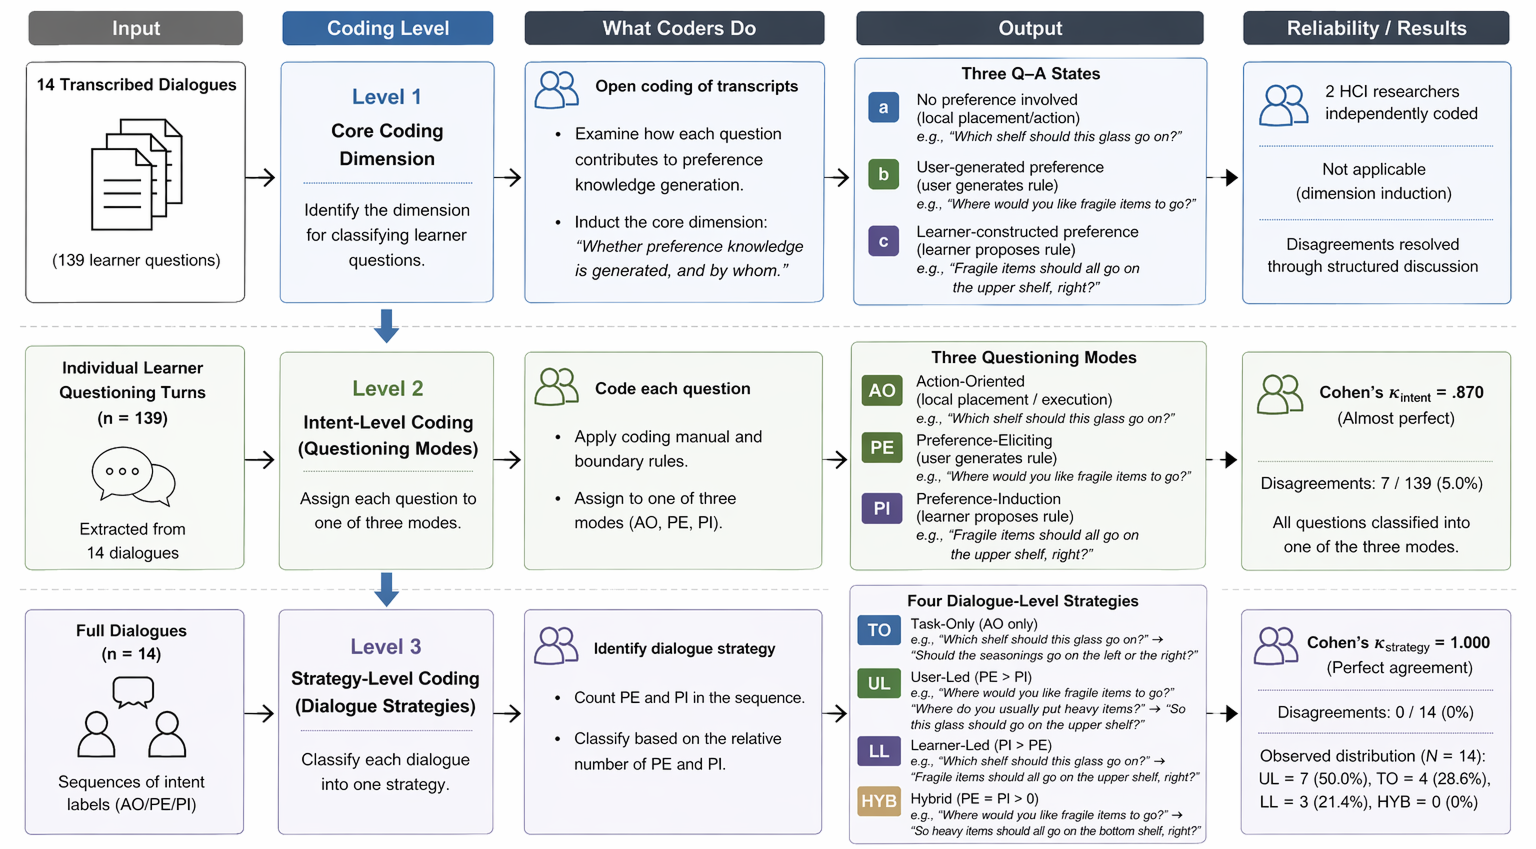
\includegraphics[width=\linewidth]{img/encoding_pipeline.png}
  \caption{Three-level hierarchical coding framework. The core analytical dimension (level one) provides the operational basis for intent-level coding (level two), which assigns each question to one of three questioning modes (AO, PE, PI); the resulting intent sequence for each dialogue is then classified into a questioning strategy (level three).}
  \Description{A three-level coding pipeline that moves from raw human-human dialogue transcripts to a core coding dimension, then to intent-level questioning modes, and finally to dialogue-level questioning strategies.}
  \label{fig:annotation-pipeline}
\end{figure}

Two HCI researchers independently applied the framework to all 14 transcripts without prior discussion; disagreements were resolved through structured deliberation \citep{saldana2021coding}. Inter-rater reliability was assessed separately at the intent level and the strategy level using Cohen's $\kappa$.

\subsubsection{Coding Dimension and Questioning Modes}
\label{sec:coding-dimension}

During the open-coding phase \citep{saldana2021coding}, coders observed that the critical difference among learner questions lay not in surface intent but in how each question participated in the generation of preference knowledge. The inductive process unfolded in two steps. First, some questions were used solely to advance a specific placement or operational decision within the current task: their answers were determined by object properties, spatial constraints, or task logic, and produced no preference knowledge. Other questions produced preference rules that were transferable to subsequent objects or analogous situations. Second, among questions that did produce preference rules, the cognitive origin of rule content diverged further: some questions invited the teacher to articulate preferences, with the learner receiving the resulting rule; others had the learner first propose a rule hypothesis and submit it for teacher confirmation, correction, or rejection. Based on these two distinctions, we established \textit{who originates preference knowledge} as the core coding dimension, recognizing three question-answer states: (a)~no preference knowledge is generated, and the exchange resolves only a local placement or operational decision within the current task; (b)~the teacher generates preference-rule content, which the learner receives; and (c)~the learner independently constructs a rule hypothesis and submits it for teacher adjudication.

We adopted ``whether a transferable preference rule is produced'' as the primary operational indicator distinguishing non-preference questions from preference-oriented ones. A transferable preference rule is an organizing principle applicable to multiple objects of the same type, analogous situations, or subsequent placement decisions. Questions that produce no such rule typically resolve a local execution problem within the current task, whether for a single object or for the zone assignment of a named category. As long as a question does not ask the teacher to express a personal organizing principle or preference rule, it is classified under state~(a). We operationalize the three states as three questioning modes, each corresponding to a determinate state of preference knowledge generation with explicit coding criteria.

\textbf{Action-Oriented (AO)} questions focus on the concrete execution of the task, with the goal of clarifying a placement or operational method within the current task. The coding criterion is that the question concerns object properties, spatial arrangement, operational steps, or the zone assignment of a named category within the current task, without asking the teacher to express a personal organizing principle or preference rule. The answer confirms one local placement or operational decision, for example ``Which shelf does this glass go on?'' or ``Does the condiment go on the left side or the right?'' The learner occupies an \textbf{executor} role in AO questions; AO also constitutes the task-execution baseline against which the two preference-oriented modes are contrasted.

\textbf{Preference-Eliciting (PE)} questions aim to establish the teacher's overall inclination for a category or decision dimension. The coding criterion is that the question explicitly invites the teacher to express a preference, whether in open-ended or option-constrained form, such that the answer produces a transferable preference rule covering multiple objects, analogous situations, or subsequent placement decisions, for example ``Where would you like fragile items to go?'' or ``Do you generally prefer to keep heavy things on the top shelf or the bottom shelf?'' Rule content is generated by the teacher; the learner occupies a \textbf{receiver} role. It should be noted that ``teacher-generated'' here refers to the originator of the preference-rule content, not to who holds conversational control. The learner still initiates the question structure and determines the inquiry dimension, but the specific direction of the rule is produced by the teacher.

\textbf{Preference-Induction (PI)} questions have the learner independently infer a rule hypothesis and present it to the teacher, inviting confirmation, rejection, or revision. The coding criterion is that the learner bears the cognitive work of rule-content generation, and the hypothesis must carry rule-level coverage applicable to multiple objects of the same type, analogous situations, or subsequent placement decisions, for example ``Fragile things all go on the top shelf, right?'' or ``Heavy things all go on the bottom shelf, is that right?'' The source of the hypothesis may be prior knowledge, intuitive judgment, or accumulated dialogue observations. A yes-or-no question that confirms only a single object's placement, even if phrased in a confirmation-seeking tone, is coded AO and not PI. The fundamental distinction between PI and PE lies in the cognitive origin of rule content: in PE, rule content is generated from scratch by the teacher, and the learner is a receiver; in PI, rule content is actively constructed by the learner, and the teacher is an adjudicator. The learner occupies an \textbf{active constructor} role.

Taken together, AO, PE, and PI distinguish whether preference knowledge is absent, teacher-generated, or learner-constructed. Table~\ref{tab:questioning-modes} summarizes the coding criteria and preference knowledge construction role for each questioning mode.

\begin{table*}[t]
\centering
\caption{Three questioning modes and their coding criteria. Knowledge output and learner role are determined by the core coding dimension: who originates preference knowledge.}
\label{tab:questioning-modes}
\small
\renewcommand{\arraystretch}{1.15}
\begin{tabularx}{\textwidth}{@{} >{\raggedright\arraybackslash}p{1.3cm} >{\raggedright\arraybackslash}p{2.7cm} >{\raggedright\arraybackslash}X >{\raggedright\arraybackslash}p{2.5cm} >{\raggedright\arraybackslash}p{3.6cm} @{}}
\toprule
\textbf{Mode} & \textbf{Knowledge Output} & \textbf{Coding Criterion} & \textbf{Learner Role} & \textbf{Example} \\
\midrule
AO & None &
Question concerns object properties, spatial arrangement, operational steps, or named-category zone assignment within the current task; does not ask the teacher to express a preference rule &
Executor &
``Which shelf does this glass go on?'' \\[4pt]
PE & Present (teacher-generated) &
Question explicitly invites the teacher to express a category-level or dimension-level preference; answer produces a transferable preference rule &
Receiver &
``Where would you like fragile items to go?'' \\[4pt]
PI & Present (learner-constructed) &
Learner constructs a rule-level hypothesis and solicits teacher adjudication; hypothesis must carry rule-level coverage applicable to multiple objects or situations &
Active Constructor &
``Fragile things all go on the top shelf, right?'' \\
\bottomrule
\end{tabularx}
\end{table*}

The above framework was consolidated into a unified coding manual operationalizing the criteria and boundary rules for each mode into step-by-step guidelines for the two researchers to use independently. During coding, the K-type knowledge classification framework \citep{shin2023uncertainty} served only as a sensitizing concept to help coders identify utterances potentially involving knowledge-generation boundaries; it does not constitute a formal coding dimension of the present study.

\textbf{Inter-rater reliability.} Intent-level coding produced seven disagreements (disagreement rate = 5.0\%), distributed across three boundary types: three between AO and PE (involving zone-assignment queries for named categories), three between AO and PI (involving declarative or confirmation-seeking layout utterances), and one between PE and PI (involving a foregrounded learner hypothesis). Systematic adjudication of each boundary type yielded three decision rules: (1)~a question asking about the zone assignment of a named category within the current task space is coded AO and not PE if it does not ask the teacher to express a personal organizing principle or preference rule---PE requires the teacher to generate a transferable organizing strategy; (2)~an utterance that confirms only a specific object or local layout within the current task is coded AO and not PI---PI requires an explicit rule-level hypothesis and a verification-seeking act; (3)~if the first clause of a question proposes a learner-inferred rule and the second clause solicits teacher endorsement, the dominant speech act is coded PI. Cohen's $\kappa_1 = \mathbf{.870}$ between the two HCI coders, falling in the ``almost perfect'' range ($\kappa > .80$; \citealt{landis1977measurement}). Across all 139 learner question turns in the 14 dialogues, every turn was assigned to one of the three modes; no stable fourth intent mode emerged during coding.

\subsubsection{Questioning Strategy Identification}
\label{sec:strategy-id}

After intent-level coding, we used the complete intent-label sequence for each dialogue as the unit of analysis to identify dialogue-level dominant questioning strategies. Strategy classification was based not on the local function of individual questions but on the relative counts of PE and PI, the two preference-oriented question types, across the full dialogue. PE indicates that the teacher was invited to generate preference content; PI indicates that the learner actively constructed a preference hypothesis and submitted it for teacher adjudication. The relative counts of the two therefore reflect the distribution of initiative in preference rule generation between the teacher side and the learner side.

Based on the relative counts of PE and PI, we define four logical configurations. When both counts are zero (the sequence contains only AO), the dialogue is classified as Task-Only (TO). When the teacher side exceeds the learner side (PE count greater than PI count), the dialogue is classified as User-Led (UL). When the learner side exceeds the teacher side (PI count greater than PE count), the dialogue is classified as Learner-Led (LL). When the teacher side equals the learner side and neither is zero (PE count equals PI count, both greater than zero), the dialogue is classified as Hybrid (HYB). The four strategy configurations and their distribution in the HHI corpus are summarized in Table~\ref{tab:hhi-strategies}. TO, UL, and LL were empirically observed; HYB is a logical configuration derivable from the classification rules but was not observed in the current HHI data.

\begin{table*}[t]
\centering
\caption{Dialogue-level questioning strategies and their distribution in the HHI corpus ($N = 14$ dyads). HYB is a theoretically derived configuration not observed in the current HHI data.}
\label{tab:hhi-strategies}
\small
\renewcommand{\arraystretch}{1.15}
\begin{tabularx}{\textwidth}{@{} >{\raggedright\arraybackslash}p{2.7cm} >{\raggedright\arraybackslash}p{4.2cm} >{\raggedright\arraybackslash}X >{\centering\arraybackslash}p{1.4cm} @{}}
\toprule
\textbf{Strategy} & \textbf{Classification Rule} & \textbf{Example Sequence} & \textbf{$N$ (\%)} \\
\midrule
TO (Task-Only) &
PE $= 0$ and PI $= 0$; the sequence contains only AO questions and remains at item-level placement confirmation. &
\begin{minipage}[t]{\linewidth}\raggedright
``Which shelf for this glass?'' (AO)\par
$\rightarrow$ ``Condiment left or right?'' (AO)\par
$\rightarrow$ ``Horizontal or upright?'' (AO)\par
$\rightarrow$ ``Can this go here?'' (AO)
\end{minipage} &
4 (28.6\%) \\[4pt]
UL (User-Led) &
PE $>$ PI; the learner primarily invites the teacher to generate category-level preference rules, with AO used for execution. &
\begin{minipage}[t]{\linewidth}\raggedright
``Where should fragile items go?'' (PE)\par
$\rightarrow$ ``Where do heavy things go?'' (PE)\par
$\rightarrow$ ``So this glass goes on the top shelf?'' (AO)\par
$\rightarrow$ ``Soy sauce on the bottom shelf?'' (AO)
\end{minipage} &
7 (50.0\%) \\[4pt]
LL (Learner-Led) &
PI $>$ PE; the learner primarily constructs rule hypotheses from accumulated evidence and submits them for teacher adjudication. &
\begin{minipage}[t]{\linewidth}\raggedright
``Which shelf for this glass?'' (AO)\par
$\rightarrow$ ``Where does the soy sauce go?'' (AO)\par
$\rightarrow$ ``Fragile things all go on the top shelf, right?'' (PI)\par
$\rightarrow$ ``Heavy things go on the bottom, right?'' (PI)
\end{minipage} &
3 (21.4\%) \\[4pt]
HYB (Hybrid) &
PE $=$ PI $> 0$; teacher-generated and learner-constructed preference rules appear in balanced proportions. &
\begin{minipage}[t]{\linewidth}\raggedright
``Where should fragile items go?'' (PE)\par
$\rightarrow$ ``Heavy things go on the bottom, right?'' (PI)\par
$\rightarrow$ ``What goes on the top shelf?'' (PE)\par
$\rightarrow$ ``Cans go on the bottom, right?'' (PI)
\end{minipage} &
0 (0.0\%) \\
\bottomrule
\end{tabularx}
\end{table*}

Applying the above rules to all 14 dialogues, three strategies were empirically observed: UL in 7 dialogues (50.0\%), TO in 4 (28.6\%), and LL in 3 (21.4\%). UL was the most common strategy, indicating that the majority of learners preferred to cede initiative in preference-content generation to the teacher, first establishing category-level rules through PE questions and then executing specific placements within the resulting rule framework. TO was intermediate, with learners remaining at the task-execution level throughout and preference rule construction entirely absent; the learner acted primarily as an executor. LL was least frequent yet reflects the most proactive preference knowledge construction stance: learners in this group first constructed rule hypotheses based on object properties, task observations, or prior dialogue evidence, and submitted these for teacher adjudication rather than waiting for the teacher to volunteer preference rules.

The coexistence of all three strategies under identical task conditions indicates that the distribution of preference-construction initiative reflects genuine individual strategic variation rather than a direct product of the task context. HYB did not emerge naturally in the current HHI corpus and is therefore not reported as an empirical strategy type in the HHI results. However, HYB is a theoretical configuration derivable from the combination rules of PE and PI, representing a balanced combination of teacher-generated and learner-constructed preference rule sources. As a theoretical extension, HYB will be considered in the agent strategy design in Section~\ref{sec:system-design}.

\textbf{Inter-rater reliability.} The two coders reached full agreement on strategy classification across all 14 dialogues (Cohen's $\kappa_2 = \mathbf{1.000}$; disagreements = 0). This result indicates that, once intent labels are determined, strategy classification based on the relative counts of PE and PI is highly reproducible. The primary uncertainty is therefore concentrated at intent-level boundary cases rather than in the strategy-level classification rules.

This coding framework provides the empirical basis for the agent strategy design in Section~\ref{sec:system-design}. Specifically, AO, PE, and PI are transferred as the agent's question generation modes; TO, UL, LL, and HYB are transferred as dialogue-level strategy configurations for subsequent system implementation and user study comparisons.

% =============================================================================
\section{System Design}
\label{sec:system-design}
% =============================================================================
{\revstart

\subsection{Problem Formulation}
\label{sec:task-formulation}

We formulate household rearrangement as a budgeted preference-learning problem in which the agent must learn a user's organizing preferences through dialogue before acting. A task instance is defined by a tuple $(R, \mathcal{C}, \mathcal{O}_s, \mathcal{O}_u)$, where $R$ is the room type, $\mathcal{C} = \{c_1, \dots, c_M\}$ is the set of available receptacles, and $\mathcal{O}_s$ and $\mathcal{O}_u$ are the sets of \textit{seen} and \textit{unseen} objects, respectively. Seen objects are available during the interaction and can be queried about directly. Unseen objects are held out from dialogue: the agent never asks about them explicitly and must place them by generalizing from learned preferences. The agent may ask at most $B$ questions before producing placements for all objects.

This framing makes the central constraint explicit: the agent has only a limited number of opportunities to ask, yet must recover preferences that are often abstract, tacit, and only partially articulable. At each turn $t \in \{1, \dots, B\}$, the system observes the current preference state $\mathcal{S}_t$, selects a question $q_t$ according to the active strategy, receives the user response $a_t$, converts it into structured evidence, and produces an updated state $\mathcal{S}_{t+1}$. After dialogue terminates, the system outputs a placement function $\hat{y}: \mathcal{O}_s \cup \mathcal{O}_u \rightarrow \mathcal{C}$. The key challenge is therefore not only \textit{what} to ask but also \textit{at what level of abstraction}---object-specific or category-level---to ask it.

\subsection{PrefQuest: A Structured Preference Learning Framework}
\label{sec:prefquest}

\begin{figure*}[t]
  \centering
  \includegraphics[width=\textwidth]{img/framework.png}
  \caption{Overview of the \textsc{PrefQuest} framework. The per-turn dialogue loop (dashed border) operates as follows: the \textit{Strategy Controller} selects a questioning mode (AO, PE, or PI) conditioned on the current Structured Preference State~$\mathcal{S}_t$; the \textit{Pattern Proposer} instantiates the selected mode as a natural-language question; the user responds; and the \textit{Preference Updater} interprets the answer and updates $\mathcal{A}^+$, $\mathcal{P}^+$, $\mathcal{A}^-$, $\mathcal{P}^-$, and $\mathcal{U}$ accordingly. Objects newly entering $\mathcal{A}^+$ are placed immediately; remaining unresolved objects are handled by the \textit{Placement Planner} upon dialogue termination, which assigns receptacles in priority order: (1)~$\mathcal{P}^+$ rule-based match, (2)~$\mathcal{A}^+$ semantic analogy, (3)~commonsense fallback.}
  \Description{A system architecture diagram for PrefQuest showing a dialogue loop with a strategy controller selecting AO, PE, or PI questioning modes, a pattern proposer, user response, preference updater, structured preference state, immediate placement for confirmed actions, and a final placement planner.}
  \label{fig:system-architecture}
\end{figure*}

Building on the HHI-derived questioning modes and dialogue-level strategies summarized in Tables~\ref{tab:questioning-modes} and~\ref{tab:hhi-strategies}, we present \textsc{PrefQuest}, a framework for proactive preference learning in household rearrangement. Its purpose is to make the transfer from human learner questioning to agent-initiated questioning explicit and controllable. The framework operationalizes the three HHI questioning modes (AO, PE, PI) as agent-side questioning modes, and composes them into deterministic dialogue-level questioning strategies (TO, UL, LL, HYB). This design allows strategy composition to vary independently of the placement inference pipeline, so that later performance differences can be attributed to questioning design rather than to unrelated implementation choices.

The central design claim of \textsc{PrefQuest} is that preference learning should be driven by proactive questioning organized around structured evidence accumulation, rather than by passive interpretation of raw dialogue alone. The framework operationalizes this claim through two components. First, it maintains a structured preference representation that explicitly separates object-level evidence, category-level rules, and negative feedback, enabling hierarchical reasoning over accumulated preference information. Second, it treats questioning strategy as a controllable layer that selects among AO, PE, and PI modes according to deterministic scheduling rules. We hypothesize that without explicit separation of object-level evidence ($\mathcal{A}^+$) from category-level rules ($\mathcal{P}^+$), an LLM placer may struggle to reliably apply rules to unseen objects because rules and instances blur in raw dialogue---a prediction we test against the Raw LLM baseline in Section~\ref{sec:study1}.

\subsubsection{Framework Overview}

Figure~\ref{fig:system-architecture} illustrates the overall framework. \textsc{PrefQuest} operates as a per-turn dialogue loop governed by two inputs: a fixed \textit{questioning strategy} (TO, UL, LL, or HYB) that constrains which modes are available, and a dynamic \textit{Structured Preference State}~$\mathcal{S}_t$ that records what has been learned so far. The Structured Preference State is the central hub: it is updated after every turn, drives the next mode selection, and provides the hierarchical evidence base for final placement inference once the dialogue ends.

\subsubsection{Preference State Representation}
\label{sec:structured-state}

Rather than relying only on raw dialogue history, the agent maintains a structured state $\mathcal{S}_t$ that separates different kinds of learned preference information:

\begin{itemize}[leftmargin=*]
    \item \textbf{Confirmed actions} $\mathcal{A}^+ = \{(o_i, c_j)\}$: specific object--receptacle pairs confirmed by the user (e.g., \textit{``the reading light goes on the nightstand''}).
    \item \textbf{Confirmed preferences} $\mathcal{P}^+ = \{(h_k, O_k, c_k)\}$: category-level organizing rules, each consisting of a natural-language hypothesis $h_k$, a set of covered objects $O_k \subseteq \mathcal{O}_s$, and optionally a target receptacle $c_k$.
    \item \textbf{Negative actions} $\mathcal{A}^-$: object--receptacle pairs explicitly rejected by the user.
    \item \textbf{Negative preferences} $\mathcal{P}^-$: category-level hypotheses rejected by the user.
    \item \textbf{Unresolved objects} $\mathcal{U}_t = \mathcal{O}_s \setminus \{o : (o, \cdot) \in \mathcal{A}^+\}$: seen objects not yet assigned to a receptacle.
\end{itemize}

This representation serves two purposes. First, it enables the strategy controller to reason about what information is still missing---for example, which receptacles lack any confirmed preference---and to select the next questioning mode accordingly. Second, it provides the placement planner with a hierarchical evidence base: confirmed preferences take priority over action-based analogy, which in turn takes priority over general commonsense.

\subsubsection{Questioning Mode Implementation}
\label{sec:question-modes}

Each questioning mode is implemented as an independent LLM-based proposer module. Each module takes the current state $\mathcal{S}_t$ as input and returns a candidate question together with the object or hypothesis it is intended to probe:

\begin{itemize}[leftmargin=*]
    \item \textbf{Action-Oriented (AO).} AO asks about the placement of a single specific object (e.g., \textit{``Where should the reading light go?''}), typically yielding a confirmed action $(o_i, c_j)$. The AO proposer selects a target object from $\mathcal{U}_t$, prioritizing objects associated with receptacles not yet covered by any confirmed preference or action. Once all receptacles have at least one confirmed preference, the proposer shifts to \textit{boundary-probe} mode, targeting objects whose category membership is ambiguous under the current rules.
    \item \textbf{Preference-Eliciting (PE).} PE asks directly about the user's organizing habits for a category of objects (e.g., \textit{``How do you usually organize electronic accessories?''}). A successful PE turn yields a confirmed preference $(h_k, O_k, c_k)$ covering multiple objects. The PE proposer operates in two stages: it first groups objects in $\mathcal{U}_t$ by shared semantic attributes to build candidate \textit{(hypothesis, covered-objects)} pairs; it then selects the candidate that best covers currently under-supported receptacles and generates the corresponding category-level question.
    \item \textbf{Preference-Induction (PI).} PI proposes a rule inferred from previously confirmed actions and asks the user to confirm, refine, or reject it (e.g., \textit{``I noticed you placed the remote and speaker both in the media drawer---do you generally keep handheld electronics there?''}). The PI proposer examines $\mathcal{A}^+$, identifies receptacles supported by multiple confirmed objects, and generates a testable category-level hypothesis. PI is triggered only when at least two confirmed actions point to the same receptacle, ensuring the proposed hypothesis has evidential support before the user is asked to generalize.
\end{itemize}

Figure~\ref{fig:pattern-cards} illustrates all three modes as parallel pipelines across five stages---evidence source, proposer decision, generated question, user response, and state update---highlighting how the modes differ in prior evidence required, internal proposer logic, and which fields of the Structured Preference State are updated.

\begin{figure*}[t]
  \centering
  \includegraphics[width=\textwidth]{img/pattern-cards.png}
  \caption{The three questioning modes in \textsc{PrefQuest} (AO, PE, PI), shown as mode-specific pipelines across five stages: evidence source, proposer decision, generated question, user response, and state update target. The \textit{proposer decision} stage highlights the key differences between modes: the AO proposer selects a target object by receptacle-coverage priority and switches to boundary-probe mode once all receptacles are covered; the PE proposer operates in two stages, first building candidate \textit{(hypothesis, covered-objects)} pairs from semantic groupings of $\mathcal{U}_t$, then selecting the candidate that covers the most receptacle gaps; the PI proposer is gated by a trigger condition---at least two confirmed actions must point to the same receptacle---before it induces a generalizable hypothesis. These differences in evidence source and proposer logic explain why PE turns yield multi-object $\mathcal{P}^+$ rules whereas AO turns yield single-object $\mathcal{A}^+$ entries.}
  \Description{A row-based diagram comparing AO, PE, and PI questioning modes across evidence source, proposer decision, generated question, user response, and state update target.}
  \label{fig:pattern-cards}
\end{figure*}

\subsubsection{Strategy Execution}
\label{sec:strategies}

A \textit{questioning strategy} determines which modes are available and in what order they are deployed across the budget. All four strategies are implemented as deterministic, rule-based schedulers to ensure reproducibility and to preserve a direct mapping to the HHI strategy definitions.

\paragraph{Task-Only (TO).} TO uses only AO questions throughout the entire budget, resolving one seen object's placement per turn. TO serves as a strong baseline: it makes no attempt to learn generalizable rules, but accumulates maximal concrete evidence for the placement planner's analogy step.

\paragraph{User-Led (UL).} UL begins with PE questions to discover category-level organizing rules, prioritizing receptacles that lack any confirmed preference. Once all receptacles have at least one confirmed rule, the strategy switches to AO questions that probe \textit{boundary cases}---objects whose category membership is ambiguous given the current rules. This top-down approach mirrors the human User-Led pattern observed in HHI.

\paragraph{Learner-Led (LL).} LL begins with AO questions to collect concrete placement evidence. After accumulating at least two confirmed actions at the same receptacle, LL triggers a PI question that proposes a generalizable hypothesis inferred from the observed placement pattern and asks the user to confirm, refine, or reject it. This bottom-up ``do-and-induce'' loop mirrors the Learner-Led pattern observed in HHI.

\paragraph{Hybrid-All (HYB).} HYB operationalizes the logical Hybrid configuration from Section~\ref{sec:hhi} as an adaptive reference condition combining all three modes. It selects among them based on state signals: after each PE question, the system evaluates whether the resulting preference is ``strong'' (covers $\geq$2 objects and resolves to a specific receptacle); if weak, the system falls back to AO. When unsummarized confirmed actions accumulate ($\geq$2 without a corresponding rule), the system triggers PI.

Figure~\ref{fig:strategy-timeline} visualizes how the four strategies allocate their budgets across turns.

\begin{figure*}[t]
  \centering
  \includegraphics[width=\textwidth]{img/strategy-timeline.png}
  \caption{Budget allocation across the four questioning strategies at $B{=}5$. Each cell represents one dialogue turn, colored by questioning mode (AO, PE, PI). The annotation panel illustrates the resulting Structured Preference State after five turns for UL versus TO: UL accumulates transferable category rules ($\mathcal{P}^+$) whereas TO accumulates only object-level actions ($\mathcal{A}^+$), explaining UL's superior generalization to unseen objects.}
  \Description{A timeline diagram showing how TO, UL, LL, and HYB allocate five dialogue turns across AO, PE, and PI questioning modes, with an annotation comparing the resulting preference states for UL and TO.}
  \label{fig:strategy-timeline}
\end{figure*}

\subsubsection{State Update}
\label{sec:state-update}

After each question--answer exchange, the \textit{Preference Updater} interprets the user's natural-language answer and updates $\mathcal{S}_t$ through one of three paths. The path is determined by the questioning mode recorded at proposal time, so no additional LLM call is needed to re-identify the mode from raw text:

\begin{itemize}[leftmargin=*]
    \item \textbf{AO answer interpretation:} The LLM classifies the answer as a direct placement (confirmed action), an exclusion (negative action), or an incidental general rule (confirmed preference).
    \item \textbf{PE answer interpretation:} The LLM extracts a category-level rule, identifies covered objects, and determines acceptance or rejection. Accepted rules are added to $\mathcal{P}^+$; rejected hypotheses to $\mathcal{P}^-$.
    \item \textbf{PI answer interpretation:} The LLM determines whether the user confirmed, refined, or rejected the proposed hypothesis. A special \textit{rule-with-exception} case handles partial confirmation where one object deviates from the general rule (e.g., \textit{``All electronics go in the media drawer, except the phone charger which stays on the desk''})---the confirmed rule is added to $\mathcal{P}^+$ while the exception is recorded as a negative action.
\end{itemize}

After each update, $\mathcal{U}_t$ is recomputed by removing objects appearing in confirmed actions. Any object newly entering $\mathcal{A}^+$ is placed immediately, while objects resolved only via $\mathcal{P}^+$ rules are deferred to the Final Placement Planner at dialogue end. All interpretations are generated through a single LLM call with element-specific prompts that enforce structured output.

\subsubsection{Placement Inference}
\label{sec:final-planner}

Upon dialogue termination, the \textit{Final Placement Planner} is invoked to assign receptacles to objects not resolved through real-time execution during the dialogue: unresolved seen objects in $\mathcal{U}_B$ and all unseen objects in $\mathcal{O}_u$. Resolution proceeds in two stages:

\paragraph{Seen object placement.} For each unresolved seen object $o \in \mathcal{U}_B$, the planner applies evidence in priority order: (1)~confirmed preferences---if $o$ fits a preference category, assign it to that category's receptacle; (2)~confirmed action analogy---find the most semantically similar confirmed object and apply the same receptacle; (3)~general reasoning fallback. Negative actions $\mathcal{A}^-$ are respected as hard constraints throughout.

\paragraph{Unseen object placement.} For each unseen object $o \in \mathcal{O}_u$, the planner follows the same priority but with emphasis on attribute-based matching: material, size, power source, and usage context determine which confirmed preference best fits the unseen object. When multiple preferences could match, the planner uses distinguishing attributes to select the most specific match.

This two-stage design prioritizes confirmed evidence over general commonsense knowledge, which is particularly important in personalized household tasks where individual preferences may diverge from normative defaults.

\subsection{Implementation}

\textsc{PrefQuest} is implemented as a modular Python pipeline in which each component corresponds directly to a framework module. The Structured Preference State is maintained as a typed JSON object, updated in place after every turn and passed as context to all downstream modules. The Strategy Controller is implemented as a deterministic rule-based scheduler that produces a one-sentence guidance string for the Pattern Proposer without making any LLM call itself; this keeps the control logic transparent and reproducible.

For all LLM-based modules---the Pattern Proposer, Preference Updater, and Final Placement Planner---we used GPT-5-Chat with temperature set to 0.0 throughout, promoting consistent outputs across all turns and conditions. All modules enforce structured outputs via JSON-mode generation with schema validation. The pipeline is orchestrated using the LangChain Python library~\cite{langchain2023}.

The following section empirically tests three predictions implicit in this design: (i) that strategy composition produces measurable differences in unseen-object PSR; (ii) that UL's top-down rule elicitation transfers better to novel objects than TO's object-by-object resolution; and (iii) that the structured preference state contributes beyond the LLM backbone, as tested against a matched Raw LLM baseline.

\revend}

% =============================================================================
\section{Simulation-Based Evaluation of Questioning Strategies}
\label{sec:study1}
% =============================================================================
{\revstart

Strategy composition is the key variable in \textsc{PrefQuest}: the four strategies share the same model, oracle, and task structure but differ in how they allocate a limited question budget. Whether this difference in composition produces measurable differences in preference satisfaction rate, and how each strategy's advantage accumulates across budgets from 1 to 10, can only be cleanly isolated through controlled simulation. We therefore evaluated all conditions across 102 household episodes, holding all factors constant except strategy.

\subsection{Experimental Setup}

\subsubsection{Dataset}

We constructed a dataset of 102 household episodes spanning three room types: living rooms (34 episodes), bedrooms (34 episodes), and kitchens (34 episodes). Each episode contains 12 seen objects, 16--24 unseen objects ($M = 19.1$), and 4--6 receptacles ($M = 5.1$). The asymmetric split---more unseen than seen objects---provides a rigorous test of generalization: strategies must extrapolate from limited evidence to a substantially larger set of novel objects.

Each episode includes annotator-authored natural-language notes describing the user's organizing principles. These notes serve as ground truth for the simulated oracle's responses but are never directly revealed to the agent; the agent may discover their content only through dialogue. Every receptacle has at least one seen object assigned to it, ensuring that all strategies have an equal opportunity to discover evidence for every receptacle.

Table~\ref{tab:dataset-sample} presents a representative living-room episode illustrating the dataset structure. The five annotator notes define category-level organizing rules (e.g., ``portable electronics, game controllers, and optical disc cases go to the media drawer''), which apply directly to specific seen objects and generalize to unseen objects such as \textit{portable e-reader}. A strategy that discovers such a rule via a single PE question can correctly place multiple objects, whereas a strategy that resolves them one-by-one via AO questions spends multiple budget turns on the same information.

\begin{table}[t]
\centering
\small
\caption{A representative living-room episode from the dataset. The agent observes the room type, receptacles, and seen objects during interaction; annotator notes and unseen objects are hidden. Every receptacle has at least one seen object, ensuring all strategies have evidence to discover each organizing rule.}
\label{tab:dataset-sample}
\begin{tabularx}{\linewidth}{@{} l X @{}}
\toprule
\textbf{Room} & Living room \\
\textbf{Receptacles} & display shelf, center table, media drawer, sofa, decorative basket \\
\midrule
\multicolumn{2}{@{}l}{\textbf{Seen objects} (visible during interaction)} \\
& hardcover novel, hardcover design annual, encyclopedia volume $\to$ \textit{display shelf} \\
& coasters for drinks, travel photo book $\to$ \textit{center table} \\
& solar-powered lantern, battery-powered game controller, rechargeable projector remote $\to$ \textit{media drawer} \\
& cotton reading pillow $\to$ \textit{sofa} \\
& plastic puzzle case, dried lavender bundle, vintage magazine stack $\to$ \textit{decorative basket} \\
\midrule
\multicolumn{2}{@{}l}{\textbf{Unseen objects} (hidden; placement must be inferred)} \\
& portable e-reader, hardcover art book, puzzle tin, daily crossword book, velvet throw pillow, \ldots~(17 total) \\
\midrule
\multicolumn{2}{@{}l}{\textbf{Annotator notes} (oracle ground truth; never shown to agent)} \\
& \textit{``Large, flat, or framed items meant for viewing or reading go to the display shelf.''} \\
& \textit{``Small books and drink accessories used during relaxation go to the center table.''} \\
& \textit{``Portable electronics, game controllers, and optical disc cases go to the media drawer.''} \\
& \textit{``Soft textiles and cushions for sitting comfort go to the sofa.''} \\
& \textit{``Miscellaneous items and loose accessories needing temporary storage go to the decorative basket.''} \\
\bottomrule
\end{tabularx}
\end{table}

\subsubsection{LLM-Based Oracle}

We employed an LLM-based \textit{Natural User Oracle} that simulates a cooperative household member. Given a question, the oracle generates a natural-language answer grounded in the episode's annotator notes and ground-truth placements. Unlike a simple lookup table, the oracle produces varied, realistic responses that may include partial information, category-level rules, or exceptions---reflecting the complexity of real human answers. The oracle is constrained to: (1)~never directly quote or paraphrase the annotator notes; (2)~use exact receptacle names from the provided list; (3)~maintain consistency with previous answers in the dialogue history; and (4)~honestly state when no specific organizing rule applies.

To assess oracle quality, we manually inspected a random sample of 50 oracle responses across room types and question elements, evaluating each response for (a)~faithfulness to the annotator notes, (b)~internal consistency with prior answers in the same episode, and (c)~naturalness in phrasing. All 50 responses met criteria (a) and (b); occasional minor phrasing inconsistencies were observed but did not affect the factual content of the answer.

\subsubsection{Conditions and Evaluation Metrics}

We evaluated six conditions: four questioning strategies (TO, UL, LL, HYB) and two baselines. The \textit{No Question} baseline ($B=0$) relies entirely on the LLM's commonsense knowledge without any user interaction, establishing a lower performance bound. The \textit{Raw LLM} baseline uses the same underlying model but replaces the entire \textsc{PrefQuest} pipeline with a minimal two-step procedure: a free-form LLM questioner generates one placement-related question per turn (given only room context, object lists, and prior Q\&A history, with no element constraints or structured state), and after budget exhaustion, a separate LLM placer reads the raw dialogue history to output placements without any structured evidence hierarchy. This baseline isolates the contribution of the full \textsc{PrefQuest} framework---strategy scheduling, structured state, and evidence-based planner---against a pure end-to-end LLM approach using the same oracle and the same question budget.

Each strategy was evaluated at budget checkpoints $B \in \{1, 2, \dots, 10\}$. For efficiency, each episode was run once up to $B_{\max}=10$, with the structured state evaluated at each checkpoint. The primary model was GPT-5-Chat (102 episodes, all conditions); Qwen3-8B served via Ollama was used for cross-model validation and is reported in Appendix~\ref{app:qwen3}.

For each episode and budget, we computed a unified \textit{Preference Satisfaction Rate} (PSR) over a target object set~$\mathcal{O}$:
\begin{equation}
\label{eq:psr}
\mathrm{PSR}(\mathcal{O}) = \frac{1}{|\mathcal{O}|}\sum_{o \in \mathcal{O}} \mathbf{1}\!\left[\hat{y}(o)=y(o)\right],
\end{equation}
where $y(o)$ is the ground-truth receptacle for object~$o$. Setting $\mathcal{O}=\mathcal{O}_s$ yields \textit{seen PSR}; setting $\mathcal{O}=\mathcal{O}_u$ yields \textit{unseen PSR}. We report mean PSR $\pm$ standard error across 102 episodes. Unseen PSR is the primary metric, as it directly tests whether a strategy learns transferable preferences rather than object-level facts. Between-strategy comparisons were conducted using paired Wilcoxon signed-rank tests, with Bonferroni correction applied for multiple comparisons.

\subsection{Results}

\subsubsection{Effect of Questioning Strategy on Placement Accuracy}

Table~\ref{tab:study1-results} presents the main results at selected budget checkpoints. Figure~\ref{fig:ablation-curves} shows the full accuracy curves across all budgets.

\begin{table*}[t]
\centering
\caption{Preference satisfaction rate (PSR, \%, $M \pm SE$) at selected budget checkpoints, evaluated with GPT-5-Chat ($n=102$ episodes). Bold indicates the highest unseen PSR among the four strategies at each budget. Full Qwen3-8B results are reported in Appendix~\ref{app:qwen3}.}
\label{tab:study1-results}
\begin{tabular}{l cc cc cc cc cc}
\toprule
 & \multicolumn{2}{c}{$B=0$} & \multicolumn{2}{c}{$B=1$} & \multicolumn{2}{c}{$B=3$} & \multicolumn{2}{c}{$B=5$} & \multicolumn{2}{c}{$B=10$} \\
\cmidrule(lr){2-3} \cmidrule(lr){4-5} \cmidrule(lr){6-7} \cmidrule(lr){8-9} \cmidrule(lr){10-11}
\textbf{Condition} & Seen & Unseen & Seen & Unseen & Seen & Unseen & Seen & Unseen & Seen & Unseen \\
\midrule
No Question & 68.9{\scriptsize$\pm$2.0} & 67.5{\scriptsize$\pm$2.1} & --- & --- & --- & --- & --- & --- & --- & --- \\
Raw LLM     & --- & --- & 59.7{\scriptsize$\pm$2.4} & 58.7{\scriptsize$\pm$2.4} & 66.8{\scriptsize$\pm$2.5} & 64.0{\scriptsize$\pm$2.4} & 72.3{\scriptsize$\pm$2.5} & 69.2{\scriptsize$\pm$2.4} & 81.2{\scriptsize$\pm$1.6} & 78.2{\scriptsize$\pm$1.6} \\
\midrule
TO          & --- & --- & 67.0{\scriptsize$\pm$2.3} & 64.7{\scriptsize$\pm$2.7} & 73.5{\scriptsize$\pm$2.4} & 69.1{\scriptsize$\pm$2.6} & 79.7{\scriptsize$\pm$2.0} & 72.7{\scriptsize$\pm$2.1} & 94.0{\scriptsize$\pm$0.9} & 79.8{\scriptsize$\pm$2.4} \\
UL         & --- & --- & 64.5{\scriptsize$\pm$2.7} & \textbf{67.7}{\scriptsize$\pm$2.2} & 70.0{\scriptsize$\pm$2.2} & 71.1{\scriptsize$\pm$2.0} & 79.8{\scriptsize$\pm$1.9} & \textbf{85.2}{\scriptsize$\pm$1.6} & 89.0{\scriptsize$\pm$1.5} & 87.1{\scriptsize$\pm$2.3} \\
LL         & --- & --- & 65.5{\scriptsize$\pm$2.7} & 63.2{\scriptsize$\pm$2.7} & 74.0{\scriptsize$\pm$2.2} & 69.7{\scriptsize$\pm$2.2} & 76.8{\scriptsize$\pm$2.1} & 71.0{\scriptsize$\pm$2.2} & 86.8{\scriptsize$\pm$1.2} & 77.4{\scriptsize$\pm$1.9} \\
HYB         & --- & --- & 62.2{\scriptsize$\pm$2.7} & 68.3{\scriptsize$\pm$2.2} & 68.3{\scriptsize$\pm$2.5} & \textbf{70.9}{\scriptsize$\pm$2.5} & 79.8{\scriptsize$\pm$1.8} & 81.8{\scriptsize$\pm$2.4} & 89.3{\scriptsize$\pm$1.3} & \textbf{87.4}{\scriptsize$\pm$1.6} \\
\bottomrule
\end{tabular}
\end{table*}

\begin{figure*}[t]
  \centering
  \includegraphics[width=0.9\textwidth]{img/ablation_gpt5chat_ep0-49_with_no_question_matched_nature.png}
  \caption{Seen (left) and unseen (right) preference satisfaction rate (PSR) as a function of question budget for four questioning strategies and the No Question baseline (dashed line). Model: GPT-5-Chat, $n=102$ episodes. Error bands show $\pm$1 SE\@. Qwen3-8B results are provided in Appendix~\ref{app:qwen3}.}
  \label{fig:ablation-curves}
\end{figure*}

Consistent with RQ3, strategy choice produced measurably different outcomes on unseen PSR. All four strategies improved seen PSR monotonically with budget, as expected when additional turns resolve additional objects. TO achieved the steepest seen-PSR gain (67.0\% at $B=1$ to 94.0\% at $B=10$), as each AO question resolves one seen object. Notably, at $B=1$, UL had slightly lower seen PSR than TO (64.5\% vs.~67.0\%), because a PE question asks about a category rather than confirming a specific object placement.

The key finding concerns unseen PSR. UL achieved 85.2\% unseen PSR at $B=5$ versus TO's 72.7\%---a gap of $+$12.5 percentage points (Wilcoxon signed-rank: $W = 94$, $p < .001$, $r = $~\textbf{TODO}). This advantage emerged as early as $B=3$ (71.1\% vs.~69.1\%) and remained significant at $B=10$ (87.1\% vs.~79.8\%, $+$7.4pp; $W = 105$, $p < .001$, $r = $~\textbf{TODO}). The unseen PSR curve of UL exhibited a characteristic elbow: rapid gain from $B=3$ to $B=5$ ($+$14.1pp), followed by sharply diminishing returns from $B=5$ to $B=10$ ($+$1.9pp). This pattern suggests that three to five well-chosen PE questions suffice to cover the major organizing rules for a typical episode, with additional questions contributing mainly to seen-object resolution.

Importantly, UL's unseen advantage did not extend to seen PSR. At $B=5$, UL and TO achieved statistically equivalent seen PSR (79.8\% vs.~79.7\%, $p = .80$); at $B=10$, TO had higher seen PSR (94.0\% vs.~89.0\%, $p = .013$), reflecting its object-by-object exhaustion of the seen set. This dissociation is consistent with the interpretation that UL's advantage is specifically attributable to the category-level rules in $\mathcal{P}^+$, not to greater coverage of seen objects.

LL achieved 71.0\% unseen PSR at $B=5$, below both TO (72.7\%) and UL (85.2\%), and 77.4\% at $B=10$, below TO (79.8\%). This finding is noteworthy: despite incorporating PI---an element designed to induce generalizable rules---LL did not outperform purely action-based TO on unseen PSR. The reason appears structural: within a budget of five questions, LL must first spend at least two AO turns at the same receptacle before PI can be triggered, leaving fewer remaining turns for rule-driven generalization. In practice, the unseen-PSR profile of LL closely resembled that of TO, with PI contributing only marginally to preference generalization under tight budgets.

HYB achieved 81.8\% unseen PSR at $B=5$ versus UL's 85.2\% ($-$3.4pp; $W = 184$, $p = .085$, $r = $~\textbf{TODO}), and 87.4\% versus 87.1\% at $B=10$ ($+$0.3pp; $W = 266$, $p = .796$, $r = $~\textbf{TODO}). Neither difference was statistically significant. This null result appears structural: because HYB's selector prefers PE whenever uncovered receptacles remain, and typical episodes contain four to six receptacles, HYB's element sequence coincides with UL's across most of the tested budget; PI fires only after category rules are already in place, too late to alter unseen PSR within $B \leq 10$.

Together, these three results indicate that category-level elicitation (PE) is the active ingredient driving generalization to unseen objects: pre-scheduling PE (UL) captures most of the benefit within $B \leq 10$, while bottom-up (LL) and adaptive (HYB) schedules either arrive at rules too late (LL) or converge to the same PE-first sequence (HYB). All strategies exceeded the No Question baseline (67.5\% unseen PSR) once the budget permitted rule accumulation.

\subsubsection{Does the Structured Preference State Contribute Beyond the LLM Backbone?}

Table~\ref{tab:study1-results} also includes the Raw LLM baseline, which asks up to $B$ questions via an unconstrained LLM but produces placements by reading raw dialogue history directly, without a structured preference state or evidence-based planner. At $B=5$, Raw LLM achieved 69.2\% unseen PSR---16.0pp below UL (85.2\%; $W = 64$, $p < .001$, $r = $~\textbf{TODO}) and 12.6pp below HYB (81.8\%). At $B=10$, Raw LLM reached 78.2\%, still below UL (87.1\%, $+$9.0pp; $W = 209$, $p < .001$, $r = $~\textbf{TODO}) and all structured strategies. Notably, Raw LLM at $B=10$ performed comparably to TO at $B=5$ (72.7\%), suggesting that doubling the question budget only partially compensates for the absence of structured state representation.

These results isolate the contribution of the \textsc{PrefQuest} framework beyond the underlying LLM: the structured preference state ($\mathcal{A}^+$, $\mathcal{P}^+$, $\mathcal{A}^-$) and evidence-based placement planner together produced a consistent and statistically significant PSR advantage, particularly for unseen objects where category-level rules must be retained and applied hierarchically. Results under Qwen3-8B (102 episodes) were consistent in direction and are reported in Appendix~\ref{app:qwen3}.

\revend}

% =============================================================================
\section{User Study}
\label{sec:study2}
% =============================================================================

Study 1 established that questioning strategy design produces measurable differences in objective placement satisfaction under controlled simulation conditions. That offline evidence, however, leaves three questions open that are inaccessible to simulation alone. First, the simulation oracle is a noise-free LLM answerer that responds in complete preference-expressive sentences; real users answer partially, revise mid-turn, and routinely under-specify the rule the agent is trying to extract. Whether the UL-over-TO advantage survives this shift in answerer behaviour is an empirical question the oracle cannot settle. Second, objective unseen PSR indexes what the agent learns, not what the user experiences: a strategy that is more accurate on the page may be perceived as more effortful, less natural, or less under the user's control---and a strategy that \textit{feels} best need not be the one that generalises best. Third, the HHI-derived questioning elements (AO, PE, PI) were validated in a human--human dyad in which the asker was also human; it remains to be shown that the same elements, once operationalised as an agent policy and delivered by a synthetic voice, are still perceived as natural and interpretable by real answerers. Study 2 therefore operationalises RQ3 (Section~\ref{sec:introduction}) through a controlled, within-subjects user study in which participants teach the autonomous \textsc{PrefQuest} agent their household organisation preferences across three strategy conditions. Specifically, Study 2 addresses three operational sub-questions corresponding to RQ3a--c:

\begin{itemize}[leftmargin=*]
  \item \textit{Evidence mechanism (RQ3a).} In real human--robot interaction, do TO, UL, and LL produce qualitatively different types of preference evidence---specifically, differing ratios of object-level confirmations ($\mathcal{A}^+$) to category-level preference rules ($\mathcal{P}^+$)---consistent with the mechanism proposed in Section~\ref{sec:introduction}?
  \item \textit{Generalization replication (RQ3b).} Does the unseen-PSR advantage of UL over TO observed in simulation replicate when questions are answered by real users rather than a simulated oracle?
  \item \textit{User experience and objective--subjective alignment (RQ3c).} Do the three strategies produce measurably different effects on teaching effort, perceived transferable understanding, and proactive questioning experience? Do objective unseen-PSR rankings and subjective strategy-preference rankings follow the same ordering, or do the two dimensions dissociate?
\end{itemize}

\subsection{Study Design}
\label{sec:study2:design}

A within-subjects design was adopted, with each participant experiencing all three strategy conditions across separate trials. A between-subjects design was considered but rejected on statistical grounds: the expected real-user effect---estimated conservatively at 60\% of the simulation effect---requires within-person comparison to achieve adequate sensitivity at a feasible sample size (see Section~\ref{sec:study2:participants}). The primary risk of a within-subjects design is order or learning effects; this risk is mitigated by the Latin-square counterbalancing scheme described below.

Three strategy conditions were tested: Task-Only (TO), User-Led (UL), and Learner-Led (LL). Each corresponds directly to a questioning pattern observed in the human--human interaction study (Section~\ref{sec:hhi}), making Study 2 a targeted test of ecological validity for HHI-grounded dialogue policies. Hybrid-All (HYB) was not included as a study condition: it is not grounded in observed human questioning behaviour, and was statistically indistinguishable from UL in simulation ($p = .085$ at $B = 5$; $p = .796$ at $B = 10$; Section~\ref{sec:study1}), providing no additional theoretical contrast. The dialogue was open-ended with no pre-specified turn limit. Participants signalled readiness to conclude verbally; the experimenter then ended the dialogue phase and advanced to the preference form. The number of dialogue turns was unconstrained and is treated as a secondary behavioural measure, allowing natural variation in dialogue length across strategy conditions to emerge as data rather than be suppressed by design.

Strategy order and scene assignment were counterbalanced jointly using a $12 \times 2$ design. Twelve orderings were constructed by crossing the six permutations of the three strategy conditions with two complementary scene assignment variants per permutation; two participants were assigned to each ordering, yielding $N = 24$ in total. This design achieves full counterbalancing: each of the twelve strategy--scene pairs (3 strategies $\times$ 4 scenes) appears with exactly three participants, and no participant encountered the same scene twice. The complete assignment table is provided in Appendix~\ref{app:latin-square}.

A key methodological decision concerns the collection of ground-truth preference data. Eliciting a full preference annotation \textit{before} the interaction would make participants aware of the complete object set in advance, reducing ecological validity and confounding workload comparisons across strategies. Instead, a post-dialogue preference form was collected \textit{after} each trial's dialogue and \textit{before} the system revealed its predicted placements. This form served as the participant's reference preference annotation for that trial, reflecting preferences as articulated following the teaching interaction and independent of any system output. All placement accuracy metrics were computed relative to this post-dialogue annotation.

The study was approved by the Institutional Review Board of Tongji University (approval reference: \textbf{[TODO: insert IRB reference number]}) and conducted in accordance with the Declaration of Helsinki. All participants provided written informed consent prior to enrolment.

Based on Study 1 findings and the theoretical framing in Section~\ref{sec:introduction}, three directional hypotheses were specified prior to data collection. Hypotheses concerning teaching effort, proactive questioning experience, and objective--subjective alignment are treated as exploratory, as no prior empirical evidence within this paper establishes a basis for directional predictions.

\begin{description}
  \item[\textbf{H1}] UL will produce higher unseen PSR than TO across user-determined dialogue lengths, replicating the direction of the simulation finding (Section~\ref{sec:study1}), but with a smaller effect size owing to the attenuation expected when real-user response variability replaces oracle simulation.
  \item[\textbf{H2}] UL will produce higher Perceived Transferable Understanding (PTU) than TO: UL guides participants to articulate category-level organising rules, which should increase the user's own sense that the agent has learned a transferable preference model; TO's item-by-item queries produce only object-level confirmations that are less likely to convey generalisation to the user.
  \item[\textbf{H3}] Objective unseen PSR rankings and subjective strategy-preference rankings (post-session comparison questionnaire) will not align across strategy conditions, indicating a dissociation between task performance and interaction experience.
\end{description}

% ANALYSIS PLAN NOTE (H3 operationalisation):
% H3 will be examined via two complementary comparisons, which capture distinct cognitive phenomena and must be
% reported and interpreted separately in the Results and Discussion:
%   (a) Preference--performance dissociation: subjective preference ranking (S1, "rank the three styles by how
%       much you liked them") vs. objective unseen PSR ranking. Tests whether users prefer the strategy that
%       actually works best for preference generalisation.
%   (b) Metacognitive accuracy: perceived-effectiveness ranking (Q1, "which style best helped the robot
%       understand your preferences?") vs. objective unseen PSR ranking. Tests whether users accurately predict
%       which strategy achieves higher unseen PSR---a separate question from hedonic preference.
% H3 is confirmed if (a) shows non-alignment. (b) is reported as a secondary exploratory finding.
% In Discussion §7, label these explicitly: "preference--performance dissociation" vs. "metacognitive accuracy",
% and discuss whether the two patterns converge or diverge.

The direction of UL versus LL on PTU is treated as exploratory (H2 is stated for UL vs. TO only): LL explicitly surfaces the agent's inductive reasoning to the user, which may increase or decrease perceived understanding depending on whether users experience the agent's hypotheses as accurate or presumptuous. Teaching Effort (TE) and Proactive Questioning Experience (PQE) differences across all three strategies are similarly treated as exploratory.

\subsection{Participants}
\label{sec:study2:participants}

A target sample of $N = 24$ was determined by \textit{a priori} power analysis (G*Power 3.1) for the primary planned pairwise comparison (Wilcoxon signed-rank test, two-tailed, $\alpha = .05$, power $= .80$). The expected effect size was estimated conservatively as Cohen's $d = 0.60$, derived from 60\% of the standardised UL--TO unseen-PSR difference observed in Study 1 ($d_{\text{simulation}} \approx 1.02$; real-user attenuation assumed). This analysis indicated a minimum required $N$ of 23; the target was set to 24 to satisfy the Latin-square counterbalancing structure ($12~\text{orderings} \times 2~\text{participants}$).

Participants were recruited from a university community. Inclusion criteria required participants to be aged 18 years or older, to report regular experience organising household items (at least once per week), and to have no prior participation in the human--human interaction study reported in Section~\ref{sec:hhi}. Prior to the experimental trials, participants completed a demographics questionnaire covering age, gender, education level, self-reported organising frequency (four-point: rarely to daily), and prior experience with robotic or voice-based assistants (single item, five-point scale). Organising frequency was retained as a covariate in sensitivity analyses of the primary outcome measure; the remaining demographics served as descriptive variables.

% TODO: Replace placeholder with actual participant demographics after data collection.
% Report: N, age M ± SD, gender distribution, education levels, organising frequency distribution, prior robot experience distribution.

\subsection{Task Scenarios and Materials}
\label{sec:study2:tasks}

Four matched household scenes were constructed as task materials: a bedroom, a kitchen, a study, and a living room. These room types were selected to represent qualitatively distinct semantic categories of household objects while remaining broadly familiar to the target participant population. Each scene was designed to satisfy the following constraints: 16 objects in total, five receptacles, three to four plausible semantic categories, at least two boundary-case objects whose category membership was genuinely ambiguous given the available receptacles, and comparable complexity across scenes as judged by the number of semantic categories and the proportion of boundary cases.

Each scene's 16 objects were pre-divided into a \textit{seen} set of eight and an \textit{unseen} set of eight. The seen set comprises objects known to the agent at the start of the interaction; the agent's questions were constrained to reference only seen objects. The unseen set comprises objects physically present in the scene and visible to the participant, but never mentioned or referenced by the agent during the dialogue. After the dialogue, the participant assigned preferences for all 16 objects; the agent was then required to predict placements for all 16, generalising from learned preferences to the eight unseen objects. The seen--unseen division was designed so that the seen set included at least one object associated with each of the five receptacles, ensuring that every strategy had an equal opportunity to discover the organising principle for each storage location. This design is directly analogous to the seen--unseen split used in Study 1, permitting quantitative comparison of PSR values across studies.

Physical scenes were assembled by the experimenter using real household objects matching each scene's item list. Object positions within the scene followed a standardised layout documented in a preparation guide. Full item lists for all four scenes, including object descriptions, semantic category assignments, and the pre-defined seen--unseen split, will be provided in a supplementary appendix after physical scene assembly is finalised. % TODO: Restore \ref{app:study2-items} once scene materials are photographed and tables confirmed.

The post-dialogue preference form presented the participant with a grid displaying all 16 objects and five receptacle options. Each object was required to be assigned to exactly one receptacle before the form could be submitted. Objects were presented in a randomised order on each trial to reduce position-based anchoring.

\subsection{System and Apparatus}
\label{sec:study2:apparatus}

The study was conducted using a custom web application developed for Study 2. The application comprised a FastAPI backend and a React frontend deployed on the experimenter's laptop. The \textsc{PrefQuest} pipeline described in Section~\ref{sec:system-design} was integrated directly into the backend, using the same strategy controllers, preference updater, and placement planner as in Study 1. The language model backend was configured identically to the GPT-5-Chat condition in Study 1 (temperature $= 0.0$), ensuring that performance differences between the two studies could be attributed to real-user answer variability rather than model changes.

Agent questions were delivered as synthesised speech via OpenAI's \texttt{tts-1} model (voice: \textit{alloy}), played through the robot's audio system. Participants provided answers verbally; the experimenter captured each response by holding a recording button on the control dashboard, triggering audio capture and transcription via OpenAI's \texttt{whisper-1} speech recognition model. The transcribed text was displayed on the experimenter's dashboard for review and, if necessary, correction before submission to the system. This experimenter-mediated transcription workflow ensured that speech recognition errors did not confound the agent's preference learning while keeping the participant's interaction channel focused on the physical robot.

The experimenter configured each trial by entering the object list and receptacle names into the dashboard prior to the trial, matching the physical scene prepared on the table. The experimenter advanced the interface between phases---scene presentation, dialogue, preference form, questionnaire, and system prediction---using a control panel visible only on the experimenter's display. A tablet was used to present the participant-facing preference form (Phase~3) and questionnaire (Phase~4); the experimenter handed the tablet to the participant at the start of each phase and collected it on completion. All interaction events were logged in real time to a JSONL file (one event per line), consistent with the logging format used in Study 1.

\begin{figure*}[t]
  \centering
  % TODO: Replace rule-box with final three-panel composite image (apparatus_composite.pdf or .png).
  % Left panel: laboratory photograph showing participant seated at table with physical scene objects
  %   and the robot; experimenter workstation visible in background (experimenter control dashboard).
  % Centre panel: screenshot of experimenter control dashboard (Phase 2) — current question text,
  %   press-and-hold STT recording button, editable transcription field for review, Submit Answer
  %   button, End Dialogue button, live PSR@k sidebar. No participant-facing display during Phase 2.
  % Right panel: screenshot of preference form interface (Phase 3, tablet) — drag-and-drop grid with
  %   16 object cards on the left and 5 receptacle buckets on the right; all-assigned gate visible.
  \noindent\rule{\linewidth}{0.5pt}\\[2.5em]
  {\large\textbf{[TODO: Apparatus composite figure — three panels]}}\\[0.8em]
  \textit{Left: laboratory setup photo \quad Centre: dialogue interface screenshot \quad Right: preference form screenshot}\\[2.5em]
  \rule{\linewidth}{0.5pt}
  \caption{Study~2 apparatus and interfaces. \textbf{Left}: The experimental setup: a participant seated at a table with 16 physical household objects arranged in the assigned scene layout and the robot as the primary interaction medium; the experimenter's control workstation is visible in the background. \textbf{Centre}: The experimenter control dashboard during Phase~2. The agent's generated question is displayed for reference; the experimenter uses a press-and-hold button to capture the participant's verbal response, reviews the speech-to-text transcription for errors, and submits the corrected text to the system; a live PSR sidebar shows current placement accuracy. No participant-facing display is active during Phase~2. \textbf{Right}: The preference form interface (Phase~3, tablet). The participant assigns all 16 object cards to one of five receptacle buckets using drag-and-drop; the Submit button is locked until all objects are assigned, preventing partial submissions.}
  % TODO: Update caption to reflect final visual layout if panel arrangement changes.
  \label{fig:study2-apparatus}
\end{figure*}

\subsection{Procedure}
\label{sec:study2:procedure}

Each session lasted approximately 60 minutes and followed a fixed protocol. Upon arrival, participants were briefed on the study, provided written informed consent, and completed the demographics questionnaire (approximately 5 minutes). During the briefing, participants were informed that the agent would predict a placement for every object in the scene---including objects it had not explicitly asked about during the dialogue---and that this full placement prediction would be revealed at the end of each trial. This task-level disclosure established a common evaluative frame across all participants without revealing the specific questioning mechanism used in any condition.

Before the formal trials, participants completed one practice trial using a bathroom scene not included in the main materials (eight objects, three receptacles). The practice trial introduced the full per-trial protocol: hearing the agent's audio questions, responding verbally, reviewing and correcting the transcription if needed, completing a reduced preference form, viewing the system prediction, and completing a brief two-item questionnaire. The experimenter remained present throughout the practice trial to answer procedural questions; no data from the practice trial were retained for analysis.

\begin{figure*}[t]
  \centering
  % TODO: Replace rule-box with final two-level procedure diagram (procedure_flow.pdf or .png).
  % Upper level (session timeline): horizontal swim-lane or timeline bar showing the full session
  %   structure left-to-right: [Consent + Demographics | ~5 min] →
  %   [Practice Trial | ~5 min] → [Trial 1 (Strategy A / Scene X) | ~15 min] →
  %   [Trial 2 (Strategy B / Scene Y) | ~15 min] → [Trial 3 (Strategy C / Scene Z) | ~15 min] →
  %   [Preference Ranking + Exit Interview | ~12 min]. Total ≈ 65 min.
  % Lower level (per-trial flow): vertical or horizontal 5-phase breakdown expanded from Trial box:
  %   [Phase 1: Scene Presentation (tablet)] →
  %   [Phase 2: Dialogue (open-ended; robot TTS → participant verbal → experimenter STT → submit;
  %     A+ → robot physical placement; participant signals readiness verbally)] →
  %   [Phase 3: Preference Form (16 objects, tablet)] →
  %   [Phase 4: Questionnaire (TE 3 items; PTU 3 items; PQE 4 items; tablet — blind to accuracy)] →
  %   [Phase 5: System Prediction (experimenter screen, confirmed vs inferred)].
  %   Annotate Phase 2 turn loop: robot question → TTS audio → participant verbal answer →
  %     experimenter press-and-hold STT → transcription reviewed → submit → robot physical placement.
  %   Show participant verbal signal + experimenter End Dialogue button as termination mechanism.
  \noindent\rule{\linewidth}{0.5pt}\\[2.5em]
  {\large\textbf{[TODO: Session + Trial procedure flow diagram — two levels]}}\\[0.8em]
  \textit{Upper: session-level timeline with approximate durations \quad Lower: per-trial five-phase breakdown}\\[2.5em]
  \rule{\linewidth}{0.5pt}
  \caption{Study~2 session structure and per-trial protocol. \textbf{Upper}: The full session timeline ($\approx$60~min), comprising an initial consent and baseline questionnaire block, one practice trial, three formal trials in a Latin-square counterbalanced order, and a final ranking and exit interview. Each formal trial is assigned a distinct strategy condition (TO, UL, or LL) and a distinct household scene. \textbf{Lower}: The five-phase structure of each formal trial. Phase~1 presents the scene layout on a tablet; Phase~2 runs an open-ended dialogue in which the robot delivers agent questions as synthesised speech, the participant responds verbally, and the experimenter captures and submits each response via a press-and-hold recording button---confirmed actions ($\mathcal{A}^+$) trigger immediate physical placement by the robot; the dialogue continues until the participant signals readiness to conclude; Phase~3 collects the post-dialogue preference form (tablet) before any system output is shown; Phase~4 administers the Teaching Effort (TE), Perceived Transferable Understanding (PTU), and Proactive Questioning Experience (PQE) questionnaires (tablet), ensuring subjective ratings are independent of accuracy knowledge; Phase~5 displays the complete placement result on the experimenter's screen---distinguishing \textit{confirmed} placements (resolved during dialogue) from \textit{inferred} placements (resolved by the Final Placement Planner)---alongside the participant's preference form assignments. The post-dialogue preference form (Phase~3) serves as the ground-truth reference for all placement accuracy metrics.}
  % TODO: Update caption timing estimates if session duration changes during piloting.
  \label{fig:study2-procedure}
\end{figure*}

Each formal trial proceeded through five phases. In Phase~1 (\textit{scene presentation}), the participant viewed a visual grid of all 16 objects and five receptacle options on a tablet and examined the corresponding physical objects on the table, signalling readiness when prepared. In Phase~2 (\textit{dialogue}), the agent generated questions according to the assigned strategy and delivered them as synthesised speech through the robot; the participant answered each question verbally. The experimenter captured the participant's response via a press-and-hold audio recording button, reviewed the speech-to-text transcription on the control dashboard, and submitted it to the system. As each submitted answer produced a confirmed action ($\mathcal{A}^+$), the robot immediately placed the corresponding object in the predicted receptacle, providing real-time physical feedback of the agent's current understanding. When the participant judged that the agent had sufficiently learned their preferences, they indicated this verbally; the experimenter then ended the dialogue phase and advanced to Phase~3. In Phase~3 (\textit{preference form}), the participant assigned all 16 objects to receptacles using a drag-and-drop interface on the tablet; all objects were required to be assigned before submission was permitted. In Phase~4 (\textit{questionnaire}), the participant completed the Teaching Effort (TE), Perceived Transferable Understanding (PTU), and Proactive Questioning Experience (PQE) instruments for that trial on the tablet. Questionnaire administration preceded any display of system output, ensuring that subjective ratings reflected the interaction process rather than knowledge of placement accuracy. In Phase~5 (\textit{system prediction}), the experimenter displayed the complete placement result on the control screen, showing the system's predicted placements alongside the participant's preference form assignments, with matches and mismatches highlighted and a summary accuracy score. Placements were visually distinguished by type: objects confirmed during dialogue (via $\mathcal{A}^+$ real-time execution) were marked as \textit{confirmed}; objects inferred by the Final Placement Planner from accumulated preference rules and action analogies were marked as \textit{inferred}.

After all three formal trials, participants completed a session-end comparison questionnaire on the tablet. This comprised (a) an overall preference ranking (1st, 2nd, 3rd) of the three strategies and an optional free-text comment, and (b) five forced-choice items (S2--S6) asking which strategy best exemplified each experiential dimension: best support for preference understanding, lowest effort, most appropriate initiative, preferred for home use, and most likely to over-assume. A semi-structured exit interview (approximately 12 minutes) then explored participants' perceptions of differences among the strategies, covering: which style felt most natural and why; which style best captured their preferences; which felt most effortful; whether any questions felt confusing, redundant, or presumptuous; and whether they would prefer a fixed or adaptive style in a real deployment. Full interview prompts are provided in Appendix~\ref{app:interview-guide}.

\subsection{Measures and Analysis}
\label{sec:study2:measures}

The primary outcome measure was \textit{unseen preference satisfaction rate} (unseen PSR), defined as the proportion of unseen objects for which the agent's predicted receptacle matched the participant's post-dialogue preference form assignment (Equation~\ref{eq:psr}, $\mathcal{O} = \mathcal{O}_u$). Unseen PSR directly tests whether a strategy learns transferable preference rules rather than object-level facts, and mirrors the primary metric used in Study 1. Secondary objective measures included seen PSR ($\mathcal{O} = \mathcal{O}_s$), total PSR ($\mathcal{O} = \mathcal{O}_s \cup \mathcal{O}_u$), discussed-item accuracy, and undiscussed-item accuracy. To enable comparison with Study~1 simulation benchmarks, unseen PSR was additionally computed at each turn $k$ (PSR@$k$), permitting learning-curve analysis independent of natural termination points.

Three subjective constructs were assessed after each trial to operationalise the three dimensions of the user experience chain introduced in Section~\ref{sec:introduction}: the effort of scaffolded preference expression, the perceived quality of the resulting preference representation, and the acceptability of the agent's proactive initiative. Full item text and scale design rationale are provided in Appendix~\ref{app:study2-questionnaire}.

\textit{Teaching Effort} (TE; 3 items, 7-pt Likert, 1 = Strongly Disagree, 7 = Strongly Agree) captured the cognitive burden of expressing preferences under each strategy. Items covered the effort of thinking carefully to answer (TE1), the effort required to articulate preferences (TE2), and perceived mental demand during teaching (TE3). TE is treated as exploratory: UL requires users to spontaneously formulate category-level rules, which may increase reflective effort relative to TO's item-by-item confirmation pattern; LL externalises induction to the agent, potentially reducing generative effort but increasing evaluative demand. No directional hypothesis is stated for TE, as these opposing forces make the net effect ambiguous.

\textit{Perceived Transferable Understanding} (PTU; 3 items, 7-pt Likert) captured whether participants felt the agent had learned a generalisable preference model rather than a set of object-level facts. PTU1 assessed global understanding of organising preferences; PTU2 assessed whether the agent appeared to have learned the \textit{logic} behind placements rather than individual locations; PTU3 assessed belief that the agent could apply learned preferences to objects it had not directly asked about. PTU2 and PTU3 are the primary items for objective--subjective comparison, as they directly parallel the unseen-PSR metric. H2 predicts UL $>$ TO on PTU; the direction of UL versus LL is exploratory (see Section~\ref{sec:study2:design}).

\textit{Proactive Questioning Experience} (PQE; 4 items, 7-pt Likert) captured participants' acceptance of the agent's proactive initiative in structuring the elicitation dialogue. PQE1 assessed whether the agent's questions helped communicate preferences; PQE2 assessed whether the level of initiative felt appropriate; PQE3 assessed comfort with the agent deciding what to ask next; PQE4 assessed whether questions felt presumptuous about the user's preferences. PQE4 is particularly diagnostic for LL, which proposes explicit rule hypotheses: users who experience the agent's inductions as accurate may rate PQE4 highly, while users who find the hypotheses incorrect may not. PQE differences across strategies are treated as exploratory.

To assess discriminant validity prior to hypothesis testing, an exploratory factor analysis (EFA; principal axis factoring, oblique rotation) will be conducted on the 10-item pool (TE~1--3, PTU~1--3, PQE~1--4); a three-factor solution is expected, with items cross-loading above .30 flagged for sensitivity analysis. Cronbach's $\alpha$ will be reported per construct per strategy condition \citep{schrum2023likert}.

All three instruments were administered on the tablet after Phase~3 (preference form) and before Phase~5 (system prediction), ensuring subjective ratings were blind to placement accuracy. After all three trials, participants completed a session-end comparison questionnaire consisting of (a) an overall preference ranking (1st, 2nd, 3rd) of the three strategies, and (b) five forced-choice items identifying, for each experiential dimension, which strategy best exemplified that dimension (best for understanding, least effortful, most appropriate initiative, preferred for home use, most likely to over-assume). This behavioural comparison supplements Likert-scale scores with inter-strategy judgements that do not suffer from between-person scale usage differences.

Objective behavioural measures from interaction logs included: turn count; question element type distribution (AO, PE, PI proportions); confirmed action count ($|\mathcal{A}^+|$) and confirmed preference count ($|\mathcal{P}^+|$) per trial, operationalising the evidence-type mechanism (RQ3a); mean participant response duration; and transcription correction rate.

Exit interview transcripts were analysed using reflexive thematic analysis \citep{braun2006using}; two researchers coded independently, then collaboratively consolidated themes. Inter-rater reliability was assessed on a 25\% random sample ($\kappa \geq .70$ threshold, set a priori).

For quantitative analysis, normality was assessed via Shapiro--Wilk. Where normality held, strategy effects were examined with one-way repeated-measures ANOVA (Greenhouse--Geisser correction) followed by pairwise $t$-tests with Holm correction ($\eta^2_p$ reported). Where normality was violated, Friedman tests were used with Wilcoxon signed-rank post-hoc tests and Holm correction (rank-biserial $r$ reported). Primary planned comparisons were UL vs. TO and LL vs. TO on unseen PSR; all other pairwise comparisons were exploratory. Organising frequency was examined as a covariate in mixed-effects models if a significant strategy main effect was observed.

\subsection{Results}

\subsubsection{Objective Performance}
% TODO: Placement accuracy (seen / unseen) per strategy with real users.
% Compare with simulation benchmarks (Section~\ref{sec:study1}) to assess
% ecological validity of simulation findings.

\subsubsection{Questionnaire Results}
% TODO: Summary statistics table (Shapiro--Wilk W, Friedman $\chi^2$ / ANOVA $F$, $p$,
% effect size) for TE (Teaching Effort), PTU (Perceived Transferable Understanding), and
% PQE (Proactive Questioning Experience) across strategy conditions (TO, UL, LL).
% Pairwise post-hoc comparisons (Wilcoxon + Holm or $t$-test + Holm) for all significant main effects.
% Report Cronbach's $\alpha$ per construct per condition in a supplementary table.
% Report session-end forced-choice frequencies (S2--S6) alongside ranking data (S1).

\subsubsection{Interview Results}
% TODO: Thematic analysis results.
% Anticipated themes: perception of strategy differences (efficient vs.\ curious vs.\
%   mechanical), task-modulated preferences, individual trait effects (dominance,
%   established organizational rules), HHI--HRI gap observations.


% =============================================================================
\section{Discussion}
\label{sec:discussion}
% =============================================================================
{\revstart

\subsection{Interpretation of Findings}

Taken together, the simulation results provide clear evidence that questioning strategy design is a consequential factor in robot Learning by Asking, addressing RQ3. The most striking finding is the large unseen-PSR gap between PE-based strategies (UL, HYB) and both TO and LL at $B=5$: UL achieved 85.2\% versus TO's 72.7\% ($+$12.5pp) and LL's 71.0\% ($+$14.2pp). This gap arises from a basic asymmetry in information efficiency: a single PE question can discover a category-level rule that immediately generalizes to multiple seen and unseen objects, whereas PI requires multiple prior AO turns to accumulate the evidence needed to propose a testable hypothesis. In practice, LL spent most of its budget on evidence gathering (AO) and only occasionally triggered PI, resulting in an unseen-PSR profile that closely resembled TO rather than UL.

One might expect that HYB---which has access to all three elements---would outperform UL by leveraging PI's evidence-based consolidation alongside PE's top-down elicitation. In practice, the two strategies were statistically indistinguishable ($p = .085$ at $B=5$; $p = .796$ at $B=10$). This structural equivalence arises because PE dominates element selection whenever uncovered receptacles remain---a condition that holds throughout the question budget in typical episodes. The theoretical benefit of combining PE and PI is therefore not realized in practice under the tested constraints. This finding suggests that multi-strategy systems should be carefully evaluated and reported, as adaptive complexity does not necessarily translate into performance gains.

Across all budget levels, every structured strategy outperformed the Raw LLM baseline by a substantial margin, despite both using the same underlying model and oracle. At $B=5$, the gap between UL and Raw LLM reached 16.0 percentage points. Two mechanisms appear to explain this advantage. First, the structured state prevents information loss: confirmed actions, category-level rules, and negative evidence are recorded explicitly, whereas raw dialogue history is susceptible to paraphrase drift and context limitations. Second, the evidence hierarchy ($\mathcal{P}^+ > \mathcal{A}^+ > \text{commonsense}$) enforces a principled prioritization that is difficult to reproduce reliably through prompt instructions alone, particularly when confirmed preferences and commonsense defaults conflict.

At a more abstract level, the performance ordering across strategies reflects a deeper principle: the \textit{abstraction level} at which a strategy solicits knowledge determines the \textit{generalization scope} of the representation it builds. Strategies that elicit rule-level knowledge (UL, via PE questions) construct representations that transfer to novel objects by design, since a category rule applies to any object matching the category. Strategies that collect instance-level facts (TO, via AO questions) build representations whose generalization depends entirely on semantic analogy---a weaker and noisier inference path. This asymmetry is not specific to household rearrangement; it reflects a more general principle in preference learning: \textit{the structure of the elicitation dialogue shapes the structure of what is learned}. While the present study establishes this principle empirically within a single domain, it suggests that the design of questioning strategies deserves first-class attention in any system that must generalise from bounded human--AI interactions to novel situations.

\subsection{Design Implications}

The present findings carry several implications for the design of preference-aware dialogue agents operating under interaction budget constraints.

\textbf{Implication 1: Prioritize category-level preference elicitation over item-by-item querying under tight budgets.} When the number of available interactions is limited (e.g., $B \leq 5$), agents should ask about abstract organizing rules before asking about individual objects. A single well-formed PE question can cover the placement logic for multiple unseen objects, whereas the same budget spent on AO questions leaves a large fraction of the object space unaddressed. This implication is most relevant in the early stages of agent deployment, when the agent has no prior model of user preferences.

\textbf{Implication 2: Design for a conservative querying horizon of three to five questions.} The unseen PSR curve of UL exhibited a characteristic elbow at $B=3$--$5$, after which additional questions yielded sharply diminishing returns ($+$1.9pp from $B=5$ to $B=10$). This suggests that a well-designed questioning strategy can cover the major organizing rules for a typical household episode in as few as three to five interactions. Agents that continue questioning beyond this point are likely to burden users without proportionate accuracy gains. Interaction budget should therefore be treated as a first-class design parameter, not an implementation detail.

\textbf{Implication 3: Use structured preference representations, not raw dialogue history.} The consistent and substantial advantage of all four structured strategies over the Raw LLM baseline indicates that a structured preference state---with explicit separation of confirmed actions, category-level rules, and negative evidence---is not merely an engineering convenience but a necessary design choice for reliable generalization. Agents relying solely on raw dialogue history may lose critical preference information across turns, particularly in long interactions where context limitations become relevant. Practitioners building preference-learning agents should prioritize explicit state representations over prompt-engineering approaches that read full conversation histories.

\textbf{Implication 4: Treat strategy selection as a function of task structure, not a fixed system parameter.} The present study focuses on placement tasks, for which the state-goal character favours front-loaded preference elicitation (UL). Prior work on human teaching in procedural tasks suggests that bottom-up, inductive patterns (LL-like) may be more natural when task execution order---rather than object placement---is the primary learning target~\cite{dai2024think,racca2018active}. Practitioners deploying preference-learning agents across diverse task types should therefore treat strategy selection as a configurable parameter informed by task structure, rather than a universal design choice. Empirical comparison of strategy effectiveness across qualitatively different task types remains an important direction for future work.
% TODO: Supplement with Study 2 findings when available.

\textbf{Implication 5: Recognise that elicitation strategy and interaction experience may optimise for different objectives.} The simulation findings identify UL as the most effective strategy for preference generalisation. However, the teaching effort (TE) of formulating category-level rules---requiring users to articulate abstract organising principles rather than respond to concrete object queries---may differ from strategies that distribute the inferential work differently, and users' sense of the agent's proactive questioning experience (PQE) is not guaranteed to track objective accuracy gains. LL's transparent inductive structure, in which the agent proposes a generalisation for the user to confirm, represents a third mode of cognitive distribution that may better support perceived agent initiative and interaction naturalness even when objective performance lags. Designers should therefore treat task performance (unseen PSR) and user experience (TE, PTU, PQE) as separable objectives, selecting strategies according to which objective is primary for a given deployment context. Where both matter, multi-phase strategies that begin with low-effort AO turns to establish rapport before transitioning to rule-level elicitation may offer a practical compromise.
% TODO: Supplement with Study 2 TE/PTU/PQE findings when available.

\subsection{Bridging Simulation and Real Interaction}

The present findings are based on a simulation study using an LLM-based oracle. An important open question is whether the observed strategy differences replicate in a user study with real participants---specifically, whether the $+$12.5pp advantage of UL over TO observed in simulation transfers when real-user answer variability (ambiguity, tangents, partial information) is introduced. Section~\ref{sec:study2} describes a planned user study designed to address this question. If the simulation findings hold with real users, they would provide strong ecological validity for the design implications above; if they do not, the discrepancies would themselves be informative about where LLM oracle assumptions break down.

\subsection{Questioning Strategy as Cognitive Labour Distribution}
\label{sec:discussion:labour}
% TODO [Study 2]: Supplement with empirical data after data collection.

The three strategies evaluated in this paper differ not only in their information-gathering efficiency but in how they distribute cognitive labour between the user and the agent. TO places the inferential burden on the agent: the user answers object-specific queries, and the agent must aggregate these facts into generalizable rules post-hoc. UL inverts this distribution, requiring the user to articulate abstract category-level principles directly---a higher cognitive demand that yields richer representations. LL occupies a third position: the agent performs the inductive reasoning (identifying patterns in accumulated evidence) and presents the result to the user for confirmation, sharing the cognitive work between both parties.

This three-way contrast maps onto a broader design question that extends beyond household rearrangement: \textit{in collaborative AI systems that must learn from bounded human input, how should the cognitive labour of preference formulation be allocated?} The present findings suggest that higher user cognitive investment (UL) produces better AI generalisation, but this relationship may not hold uniformly across users, tasks, or deployment contexts. Users who lack well-formed preferences, or who find abstract category questions cognitively demanding, may benefit more from the scaffolded inductive structure of LL, which guides them toward generalizable rules without requiring spontaneous articulation.

The distinction between strategies also has implications for \textit{perceived agency}: LL's transparent reasoning---surfacing patterns the agent has inferred from the user's own prior responses---may produce a stronger sense of collaborative understanding than UL's top-down elicitation or TO's mechanical querying. If Study 2 data reveal that LL achieves higher satisfaction ratings despite lower unseen PSR, this would provide direct empirical support for the claim that users' sense of being understood is shaped by the \textit{process} of interaction rather than its \textit{outcome} alone---a finding with broad implications for conversational AI design beyond the rearrangement domain.
% TODO [Study 2]: Replace speculative framing with empirical findings when available.
% Report organising-frequency and robot-experience moderation of strategy preference.
% Report task-property effects if multiple scene types show differential patterns.

\subsection{Limitations and Future Work}

\paragraph{Simulated oracle.} The primary limitation of the simulation study is the use of an LLM-based oracle rather than real human participants. While the oracle generates natural-language responses grounded in annotator notes, it may not fully capture the variability of human answers, including irrelevant tangents, ambiguous phrasing, or emotional responses. The planned user study (Section~\ref{sec:study2}) is designed to address this limitation directly.

\paragraph{Single domain.} All experiments were conducted in the household rearrangement domain. While the structured preference state and strategies are domain-general in principle, empirical validation in other domains (e.g., cooking assistance, workspace organization) remains future work.

\paragraph{Model dependence.} Results may vary across different LLM backbones. Cross-model validation with GPT-5-Chat suggests that the relative ordering of strategies is consistent, but absolute PSR values differ across models, reflecting differences in commonsense reasoning and instruction-following ability.
% TODO: Confirm with full GPT-5-Chat ablation results.

\revend}

% =============================================================================
\section{Conclusion}
\label{sec:conclusion}
% =============================================================================
{\revstart

The present work investigated whether questioning strategy design is a consequential factor in robot Learning by Asking for household preference learning. The three studies together indicate that how a robot organizes its questions---not merely what it asks---determines how well it learns and generalizes user preferences.

With respect to RQ1, the formative human--human study provided evidence that people naturally exhibit three distinct questioning patterns when teaching household tasks: Task-Only, User-Led, and Learner-Led, each reflecting a different organizational logic (single-layer reactive querying, top-down rule elicitation, or bottom-up evidence accumulation). These patterns were modulated by task structure, with User-Led favored for state-goal tasks and Learner-Led favored for procedural tasks.

With respect to RQ2, these HHI-derived patterns were successfully formalized as composable questioning design elements (AO, PE, PI) and composed into four controllable strategies within the \textsc{PrefQuest} framework, which separates questioning from inference through a structured preference state representation.

With respect to RQ3, strategy choice produced measurably different outcomes: the User-Led strategy achieved 85.2\% unseen PSR at $B=5$ versus Task-Only's 72.7\% ($+$12.5pp, $p < .001$), driven by the superior generalizability of category-level preference rules. Bottom-up induction (Learner-Led) offered no advantage over direct querying under tight budgets, and adaptive strategy combination (Hybrid-All) did not outperform the simpler preference-first heuristic. Structured preference state representation provided a consistent and substantial advantage over matched end-to-end LLM baselines across all budget levels.

Taken together, these results suggest that questioning strategy should be treated as a first-class design decision in robot learning systems---not as a single algorithm for resolving ambiguity, but as a macro-level choice with direct and measurable consequences for task generalization.
% TODO: Add Study 2 contribution when available.
\revend}

%%
%% The next two lines define the bibliography style to be used, and
%% the bibliography file.
\bibliographystyle{ACM-Reference-Format}
\bibliography{sample-base}


%%
%% If your work has an appendix, this is the place to put it.
\appendix

\section{K-type Categories}
\begin{table}[htbp]
\centering
\caption{K-type category \cite{shin2023uncertainty}}
\label{tab:k-type}
\begin{tabular}{lll}
\hline
\# & Categories     & Description \\
\hline
K1  & Identity         & Information about who or what a person or thing is \\
K2  & Class            & Inclusion relationships of categories \\
K3  & Attributes       & Properties or features of the object \\
K4  & Quantities       & Quantitative specifications \\
K5  & Spatial layout   & Spatial relations among entities \\
K6  & Temporal relation& Temporal information or sequences \\
K7  & Contents         & Additional detailed information \\
K8  & Procedure        & Order or method of a specific process \\
K9  & Causality        & Causal chains of events or states \\
K10 & Intention        & Motivation, aim or plan of another agent \\
K11 & Internal state   & Mental states such as preference or mood of another agent \\
\hline
\end{tabular}
\end{table}



\section{Task Materials and Layouts}
\label{app:items}

Figure~\ref{fig:layouts} shows the initial setups of the three tidying tasks. Each setup included 10--12 items distributed across a central table and 2--3 designated storage areas. The object composition and spatial layout were carefully designed to be comparable in complexity while still allowing for individual variation in preferences (e.g., categorization, accessibility, or arrangement).

\begin{figure}[t]
    \centering
    \includegraphics[width=\linewidth]{img/layout_1.png}
    \caption{Initial layouts for the three household tidying tasks: bar counter (left), study desk (middle), and office desk (right). Each scenario contains approximately 10--12 items and 2--3 storage spaces, designed with comparable complexity while preserving room for individual preferences.}
    \label{fig:layouts}
\end{figure}


\subsection{Item Lists}

\begin{table}[h]
\centering
\begin{tabular}{ll}
\toprule
\textbf{Item} & \textbf{Attributes} \\
\midrule
Plate & Black, with white bird pattern \\
Bowl & Small, white, with gold rim \\
Brush & Gray sponge brush on a stick \\
Sauce & Glass jar with red cap \\
Noodles & Instant noodle cup, red and black \\
Detergent & Bottle of yellow dish soap \\
Oil & Glass bottle of cooking oil \\
Spoon & White, ceramic \\
Sponge & Yellow, wavy shape \\
Lemon & Yellow, whole fruit \\
\bottomrule
\end{tabular}
\caption{Bar counter tidying item list.}
\end{table}

\begin{table}[h]
\centering
\begin{tabular}{ll}
\toprule
\textbf{Item} & \textbf{Attributes} \\
\midrule
Bottle & Transparent, plastic, with green cap \\
Notebook & Cork cover \\
Book & White, pink and green cover \\
Book & White cover, ``Design as Art'' \\
Fan & White, round \\
Measure & Retractable tape measure \\
Tape & Roll of black electrical tape \\
Sunglasses & Brown lenses, black frame \\
Keyboard & Black, Logitech brand \\
Basket & Silver, wire mesh \\
Bin & Blue, plastic \\
Doll & Gray, owl-shaped doll \\
\bottomrule
\end{tabular}
\caption{Office desk tidying item list.}
\end{table}


\begin{table}[h]
\centering
\begin{tabular}{ll}
\toprule
\textbf{Item} & \textbf{Attributes} \\
\midrule
Lamp & White, phone holder style \\
Mouthwash & Transparent bottle with blue \\
Toolset & Orange and transparent \\
Yogurt & White, plastic bottle \\
Baseball & White with red stitching \\
Doll & Brown, bear-shaped doll \\
Tissues & Blue and white package \\
Thermos & Light green \\
Gamecard & Green Xbox game case \\
Gamecard & Black GTA game case \\
Umbrella & Black and white striped \\
Remote & White, air conditioner remote \\
\bottomrule
\end{tabular}
\caption{Study desk tidying item list.}
\end{table}

\section{Qwen3-8B Ablation Results}
\label{app:qwen3}
Table~\ref{tab:qwen3-results} reports seen and unseen PSR for all conditions under Qwen3-8B (102 episodes). The ordering of strategies on unseen PSR is consistent with the GPT-5-Chat results reported in the main text: UL achieves the highest unseen PSR at moderate budgets, followed by HYB, while LL and TO remain lower. The absolute PSR values are lower than GPT-5-Chat across all conditions, reflecting the weaker commonsense prior of the smaller model.

\begin{table*}[h]
\centering
\caption{Seen and unseen preference satisfaction rate ($M \pm SE$) across 102 episodes for all conditions at selected budgets. Model: Qwen3-8B\@. $^\dagger$Raw LLM\@: $n=17$ episodes; full run pending.}
\label{tab:qwen3-results}
\begin{tabular}{l cc cc cc cc cc}
\toprule
 & \multicolumn{2}{c}{$B=0$} & \multicolumn{2}{c}{$B=1$} & \multicolumn{2}{c}{$B=3$} & \multicolumn{2}{c}{$B=5$} & \multicolumn{2}{c}{$B=10$} \\
\cmidrule(lr){2-3} \cmidrule(lr){4-5} \cmidrule(lr){6-7} \cmidrule(lr){8-9} \cmidrule(lr){10-11}
\textbf{Condition} & Seen & Unseen & Seen & Unseen & Seen & Unseen & Seen & Unseen & Seen & Unseen \\
\midrule
No Question      & .501{\scriptsize$\pm$.017} & .507{\scriptsize$\pm$.015} & --- & --- & --- & --- & --- & --- & --- & --- \\
Raw LLM$^\dagger$ & --- & --- & .574{\scriptsize$\pm$.041} & .574{\scriptsize$\pm$.032} & .578{\scriptsize$\pm$.041} & .607{\scriptsize$\pm$.031} & .603{\scriptsize$\pm$.047} & .631{\scriptsize$\pm$.035} & .647{\scriptsize$\pm$.045} & .692{\scriptsize$\pm$.032} \\
TO               & --- & --- & .534{\scriptsize$\pm$.017} & .505{\scriptsize$\pm$.015} & .667{\scriptsize$\pm$.015} & .553{\scriptsize$\pm$.014} & .753{\scriptsize$\pm$.012} & .587{\scriptsize$\pm$.014} & .931{\scriptsize$\pm$.006} & .631{\scriptsize$\pm$.013} \\
UL              & --- & --- & .541{\scriptsize$\pm$.018} & .520{\scriptsize$\pm$.014} & .616{\scriptsize$\pm$.016} & .560{\scriptsize$\pm$.013} & .792{\scriptsize$\pm$.017} & \textbf{.698}{\scriptsize$\pm$.014} & .874{\scriptsize$\pm$.016} & \textbf{.715}{\scriptsize$\pm$.013} \\
LL              & --- & --- & .544{\scriptsize$\pm$.017} & .501{\scriptsize$\pm$.015} & .650{\scriptsize$\pm$.015} & .548{\scriptsize$\pm$.015} & .721{\scriptsize$\pm$.013} & .572{\scriptsize$\pm$.015} & .858{\scriptsize$\pm$.009} & .615{\scriptsize$\pm$.014} \\
HYB              & --- & --- & .544{\scriptsize$\pm$.017} & .526{\scriptsize$\pm$.014} & .620{\scriptsize$\pm$.018} & .574{\scriptsize$\pm$.014} & .771{\scriptsize$\pm$.019} & .682{\scriptsize$\pm$.016} & .835{\scriptsize$\pm$.018} & .695{\scriptsize$\pm$.015} \\
\bottomrule
\end{tabular}
\end{table*}

% =============================================================================
% Appendix: Study 2 Scene Materials
% TODO: Fill in after physical scenes are assembled and photographed.
% One sub-figure per scene (bedroom, kitchen, study, living room).
% Each sub-figure: (a) photograph of physical tabletop arrangement +
%   (b) digital grid with seen/unseen annotation (solid vs. dashed outline).
% One table per scene: item name, description, category, seen/unseen assignment.
% Label to restore when content is added: \label{app:study2-items}
% =============================================================================

% =============================================================================
\section{Study 2 Counterbalancing Assignment}
\label{app:latin-square}
% =============================================================================

Table~\ref{tab:latin-square} shows the full counterbalancing scheme used in Study~2. The twelve orderings are formed by crossing the six permutations of the three strategy conditions with two scene assignment variants per permutation. Two participants were assigned to each ordering ($N = 24$ total). Each of the twelve strategy--scene pairs (3 $\times$ 4) appears in exactly three orderings, ensuring that no strategy--scene pairing is systematically over- or under-represented. Each strategy appears exactly four times in each trial position (T1, T2, T3), and each scene appears exactly nine times across the 36 trial slots (12 orderings $\times$ 3 trials).

\begin{table}[h]
\centering
\caption{Counterbalancing scheme for Study~2. Each row represents one ordering assigned to 2 participants. Scene abbreviations: Be = bedroom, Ki = kitchen, St = study, Li = living room. Each strategy--scene pair (3 strategies $\times$ 4 scenes = 12 pairs) appears in exactly 3 orderings, achieving full counterbalancing with $N = 24$.}
\label{tab:latin-square}
\begin{tabularx}{\linewidth}{@{} c >{\centering\arraybackslash}X >{\centering\arraybackslash}X >{\centering\arraybackslash}X @{}}
\toprule
\textbf{Ordering} & \textbf{Trial 1} & \textbf{Trial 2} & \textbf{Trial 3} \\
\midrule
1  & TO / Be  & UL / Ki & LL / St \\
2  & TO / Li  & UL / St & LL / Ki \\
3  & TO / Ki  & LL / Be & UL / Li \\
4  & TO / St  & LL / Li & UL / Be \\
5  & UL / Be & TO / Ki  & LL / St \\
6  & UL / Li & TO / St  & LL / Ki \\
7  & UL / Ki & LL / Be & TO / Li  \\
8  & UL / St & LL / Li & TO / Be  \\
9  & LL / St & TO / Li  & UL / Be \\
10 & LL / Li & TO / St  & UL / Ki \\
11 & LL / Be & UL / St & TO / Ki  \\
12 & LL / Ki & UL / Li & TO / Be  \\
\bottomrule
\end{tabularx}
\end{table}

% Verification: each strategy × scene pair appears exactly 3 times across 12 orderings.
% TO:  Be(1,8,12), Ki(3,5,11), St(4,6,10), Li(2,7,9)   — 3 each ✓
% UL: Be(4,5,9),  Ki(1,7,10), St(2,8,11), Li(3,6,12)  — 3 each ✓
% LL: Be(3,7,11), Ki(2,6,12), St(1,5,9),  Li(4,8,10)  — 3 each ✓

% =============================================================================
\section{Study 2 Questionnaire: Full Items and Design Notes}
\label{app:study2-questionnaire}
% =============================================================================

\subsection*{Full Item Text}

Table~\ref{tab:questionnaire-items} lists all nine per-trial questionnaire items across the three constructs. All items were administered in the fixed order CL $\to$ PU $\to$ IA; the session anchor ``In this session'' was prepended to PU and IA items to encourage condition-specific attribution and reduce rating drift across the three trials.

\begin{table}[h]
\centering
\caption{Study~2 per-trial questionnaire items. CL items use a 7-point scale (1 = Very Low, 7 = Very High); PU and IA items use a 7-point Likert scale (1 = Strongly Disagree, 7 = Strongly Agree). All items are positively worded.}
\label{tab:questionnaire-items}
\small
\begin{tabularx}{\linewidth}{@{} l l X @{}}
\toprule
\textbf{ID} & \textbf{Construct} & \textbf{Item text} \\
\midrule
CL1 & Cognitive Load & How mentally demanding was the interaction? \\
CL2 & Cognitive Load & How hard did you have to work to accomplish your level of performance? \\
CL3 & Cognitive Load & How irritated, stressed, and annoyed were you? \\
\midrule
PU1 & Perceived Understanding & In this session, the agent understood my organising preferences. \\
PU2 & Perceived Understanding & In this session, I believe the agent could predict where I would place items it did not ask about. \\
PU3 & Perceived Understanding & In this session, the agent seemed to understand not just specific items, but the general logic behind how I organise. \\
\midrule
IA1 & Interaction Agency & In this session, I felt that my answers actively shaped what the agent came to understand about my preferences. \\
IA2 & Interaction Agency & In this session, I felt that I, rather than the agent, determined what preferences the agent should learn about. \\
IA3 & Interaction Agency & In this session, I felt I had control over what conclusions the agent drew about my preferences. \\
\bottomrule
\end{tabularx}
\end{table}

\subsection*{Per-Item Rationale}

For PU, the three items target distinct levels of the transferability hierarchy: PU1 assesses global perceived understanding (surface-level comprehension); PU2 assesses object-level generalisation (whether the agent's knowledge extends to unseen items); and PU3 assesses rule-level generalisation (whether the agent appeared to grasp the underlying organising logic rather than isolated object facts). The progression from PU1 to PU3 mirrors the core claim of PrefQuest---that effective questioning should build transferable representations, not object-specific memories.

For IA, the three items target distinct dimensions of the user agency construct: IA1 assesses perceived influence on what the agent understood (input dimension); IA2 assesses perceived control over the content of the learning agenda (direction dimension); and IA3 assesses perceived control over the agent's final conclusions (output dimension). Together they operationalise agency as spanning from the user's contribution to the agent's resulting representation, without conflating agency with termination timing, which was procedurally constant across conditions.

\subsection*{Scale Design Notes}

No reverse-scored items were included. In within-subjects designs with three repeated questionnaire administrations, reverse-scored items introduce a confound: participants may fail to invert their response frame consistently across conditions, producing spuriously low inter-item correlations in particular conditions that suppress Cronbach's $\alpha$ for reasons unrelated to construct reliability. All three scales are therefore entirely positively worded.

\subsection*{Demand Characteristics and Disclosure Justification}

Participants were informed prior to the first trial that the agent would predict placements for \textit{all} objects in the scene---including those it had not asked about directly---and that they would see the full prediction result at the end of each trial. This disclosure could in principle inflate PU ratings if participants over-attribute understanding to the agent merely because they know generalisation is the intended goal.

We argue the disclosure does not introduce a confound for two reasons. First, participants were told \textit{what} the agent would attempt (predict all objects) but not \textit{how} any questioning strategy achieves this: the mechanisms by which PE questions extract category-level rules, or by which PI questions confirm induced preferences, were never described. PU ratings therefore still reflect participants' inferences from the dialogue itself, not from mechanism knowledge. Second, the disclosure was delivered identically across all three strategy conditions and all three trials, so any inflation it produces is a constant offset that cannot explain differential PU ratings across TO, UL, and LL. The disclosure thus serves to align participants' evaluative frame with the study's primary construct of interest---preference generalisation---without introducing a between-condition confound.

% =============================================================================
\section{Study 2 Exit Interview Guide}
\label{app:interview-guide}
% =============================================================================

The following prompts were used in the semi-structured exit interview conducted after all three formal trials. Interviewers were instructed to probe each prompt with natural follow-up questions and to avoid leading language. The order of prompts was fixed; probing sub-questions were at the interviewer's discretion.

\begin{enumerate}[leftmargin=*, label=\textbf{Q\arabic*.}]
  \item Which interaction style felt most natural to you, and why?
  \item Which style do you feel best captured your organizing preferences?
  \item Which style felt most effortful or demanding?
  \item Were there any questions that felt confusing, redundant, or that made incorrect assumptions about your preferences? If so, can you give an example?
  \item Looking across all three interactions, did you notice differences in how the robot approached you? How would you describe those differences in your own words?
  \item If you were to use a robot assistant for household organizing in everyday life, would you prefer it to always use one fixed questioning style, or to adapt its style over time? Why?
  \item Is there anything else you would like to share about your experience today?
\end{enumerate}

% TODO: Translate prompts into Simplified Chinese for Chinese-speaking participants if the
% study is conducted at Tongji University without English-proficient participants.
% Ensure back-translation is verified by a bilingual researcher.

\end{document}
\endinput
%%
%% End of file `sample-sigconf-authordraft.tex'.
